% !TEX TS-program = XeLaTeX
% use the following command:
% all document files must be coded in UTF-8
\documentclass[english]{textolivre}
% build HTML with: make4ht -e build.lua -c textolivre.cfg -x -u article "fn-in,svg,pic-align"

\journalname{Texto Livre}
\thevolume{19}
%\thenumber{1} % old template
\theyear{2026}
\receiveddate{\DTMdisplaydate{2025}{07}{16}{-1}} % YYYY MM DD
\accepteddate{\DTMdisplaydate{2025}{12}{31}{-1}} %XXXX
\publisheddate{\DTMdisplaydate{2026}{3}{13}{-1}}
\corrauthor{Willian Ricardo Bispo Murbak Nunes}
\articledoi{10.1590/1983-3652.2026.60366}
%\articleid{NNNN} % if the article ID is not the last 5 numbers of its DOI, provide it using \articleid{} commmand 
% list of available sesscions in the journal: articles, dossier, reports, essays, reviews, interviews, editorial
\articlesessionname{articles}
\runningauthor{Nunes et al.} 
%\editorname{Leonardo Araújo} % old template
\sectioneditorname{Daniervelin Pereira~\orcid{0000-0003-1861-3609}}
\layouteditorname{Leonardo Araújo~\orcid{0000-0003-3884-2177}}

\title{Open educational platform for problem-based learning in engineering: application of digital control in a thyristor rectifier}
\othertitle{Plataforma educacional aberta para aprendizagem baseada em problemas na engenharia: aplicação de controle digital em um retificador tiristorizado}
% if there is a third language title, add here:
%\othertitle{Artikelvorlage zur Einreichung beim Texto Livre Journal}


\author[1]{Willian Ricardo Bispo Murbak Nunes~\orcid{0000-0002-3574-7441}\thanks{Email: \href{mailto:willianr@utfpr.edu.br}{willianr@utfpr.edu.br}}}
\author[1]{Rodrigo da Ponte Caun~\orcid{0000-0003-1861-3609}\thanks{Email: \href{mailto:rodrigocaun@utfpr.edu.br}{rodricaun@utfpr.edu.br}}}
\author[1]{Winner Zavolski Queiroz~\orcid{0009-0005-1661-9742}\thanks{Email: \href{mailto:winner@alunos.utfpr.edu.br}{winner@alunos.utfpr.edu.br}}}
\affil[1]{Federal University of Technology - Paraná, Automation and Control Laboratory, Apucarana, PR, Brazil.}


\addbibresource{article.bib}
% use biber instead of bibtex
% $ biber article

% used to create dummy text for the template file
\definecolor{dark-gray}{gray}{0.35} % color used to display dummy texts
\usepackage{lipsum}
\SetLipsumParListSurrounders{\colorlet{oldcolor}{.}\color{dark-gray}}{\color{oldcolor}}

% used here only to provide the XeLaTeX and BibTeX logos
\usepackage{hologo}

% if you use multirows in a table, include the multirow package
\usepackage{multirow}
\usepackage{siunitx}

% provides sidewaysfigure environment
\usepackage{rotating}

% CUSTOM EPIGRAPH - BEGIN 
%%% https://tex.stackexchange.com/questions/193178/specific-epigraph-style
\usepackage{epigraph}
\renewcommand\textflush{flushright}
\makeatletter
\newlength\epitextskip
\pretocmd{\@epitext}{\em}{}{}
\apptocmd{\@epitext}{\em}{}{}
\patchcmd{\epigraph}{\@epitext{#1}\\}{\@epitext{#1}\\[\epitextskip]}{}{}
\makeatother
\setlength\epigraphrule{0pt}
\setlength\epitextskip{0.5ex}
\setlength\epigraphwidth{.7\textwidth}
% CUSTOM EPIGRAPH - END

% LANGUAGE - BEGIN
% ARABIC
% for languages that use special fonts, you must provide the typeface that will be used
% \setotherlanguage{arabic}
% \newfontfamily\arabicfont[Script=Arabic]{Amiri}
% \newfontfamily\arabicfontsf[Script=Arabic]{Amiri}
% \newfontfamily\arabicfonttt[Script=Arabic]{Amiri}
%
% in the article, to add arabic text use: \textlang{arabic}{ ... }
%
% RUSSIAN
% for russian text we also need to define fonts with support for Cyrillic script
% \usepackage{fontspec}
% \setotherlanguage{russian}
% \newfontfamily\cyrillicfont{Times New Roman}
% \newfontfamily\cyrillicfontsf{Times New Roman}[Script=Cyrillic]
% \newfontfamily\cyrillicfonttt{Times New Roman}[Script=Cyrillic]
%
% in the text use \begin{russian} ... \end{russian}
% LANGUAGE - END

% EMOJIS - BEGIN
% to use emoticons in your manuscript
% https://stackoverflow.com/questions/190145/how-to-insert-emoticons-in-latex/57076064
% using font Symbola, which has full support
% the font may be downloaded at:
% https://dn-works.com/ufas/
% add to preamble:
% \newfontfamily\Symbola{Symbola}
% in the text use:
% {\Symbola }
% EMOJIS - END

% LABEL REFERENCE TO DESCRIPTIVE LIST - BEGIN
% reference itens in a descriptive list using their labels instead of numbers
% insert the code below in the preambule:
%\makeatletter
%\let\orgdescriptionlabel\descriptionlabel
%\renewcommand*{\descriptionlabel}[1]{%
%  \let\orglabel\label
%  \let\label\@gobble
%  \phantomsection
%  \edef\@currentlabel{#1\unskip}%
%  \let\label\orglabel
%  \orgdescriptionlabel{#1}%
%}
%\makeatother
%
% in your document, use as illustraded here:
%\begin{description}
%  \item[first\label{itm1}] this is only an example;
%  % ...  add more items
%\end{description}
% LABEL REFERENCE TO DESCRIPTIVE LIST - END


% add line numbers for submission
\usepackage{lineno}
\usepackage{placeins}



\begin{document}
\maketitle

\begin{polyabstract}
\begin{abstract}
Engineering programs often face didactic limitations due to the high acquisition cost of laboratory equipment, which restricts the availability of hands-on activities. Consequently, practical experimentation may be limited, weakening the connection between theory and practice and potentially affecting student engagement. Furthermore, there is a notable scarcity of open educational resources that effectively integrate theory and practice in a clear and accessible manner. In response to this scenario, this study proposes and technically validates a low-cost, open-source educational platform designed to support practical, interdisciplinary teaching in power electronics, digital control, electronic circuits, and embedded systems programming. The platform is compatible with widely used academic microcontrollers, enabling the implementation of closed-loop control algorithms. In addition, the platform is positioned for use within a problem-based learning (PBL) framework as an instructional orientation. Accordingly, a replicable workflow guideline is provided, and student feedback from a student perception questionnaire is reported to characterize the learning experience. Simulation and laboratory results are obtained to validate the proposed solution in a representative application, demonstrating its feasibility for reproducible, hands-on control experiments while maintaining an open, accessible approach to replication and further development.


\keywords{Educational equipment \sep Active methodology \sep Learning methodology \sep Digital control}
\end{abstract}

\begin{portuguese}
\begin{abstract}
Cursos de engenharia frequentemente enfrentam limitações didáticas decorrentes do alto custo da aquisição de equipamentos laboratoriais, o que restringe a oferta de atividades práticas. Consequentemente, a experimentação prática pode ser limitada, enfraquecendo a conexão entre teoria e prática e potencialmente afetando o engajamento dos estudantes. Além disso, observa-se uma escassez de recursos educacionais abertos que integrem teoria e prática de forma clara e acessível. Diante desse cenário, este trabalho propõe o desenvolvimento de uma plataforma educacional de baixo custo e código aberto, projetada para apoiar o ensino prático e interdisciplinar de conceitos de eletrônica de potência, controle digital, circuitos eletrônicos e programação de sistemas embarcados. A plataforma é compatível com microcontroladores amplamente utilizados na academia, o que permite a implementação de algoritmos de controle em malha fechada. Adicionalmente, a plataforma é concebida para uso em uma estrutura de aprendizagem baseada em problemas (ABP) como orientação instrucional. Assim, é apresentado um guia de fluxo de trabalho replicável, e o retorno dos estudantes, obtido por meio de um questionário de percepção, é relatado para caracterizar a experiência de aprendizagem. Resultados de simulação e de laboratório são obtidos para validar a solução proposta em uma aplicação representativa, demonstrando sua viabilidade para experimentos de controle práticos e reprodutíveis, ao mesmo tempo em que mantém uma abordagem aberta e acessível para replicação e desenvolvimento futuro.

\keywords{Equipamento educacional \sep Metodologia ativa \sep Método de aprendizagem \sep Controle digital}
\end{abstract}
\end{portuguese}
% if there is another abstract, insert it here using the same scheme
\end{polyabstract}

\section{Introduction}\label{sec-intro}

A cornerstone of effective engineering education is the skillful integration of theory and practice, which is essential for equipping professionals to meet contemporary challenges. Practical, hands-on classes play a pivotal role in this formative process, enabling students to solidify their theoretical knowledge, engage with real-world problems, and develop critical, applied skills. However, creating meaningful practical experiences is a significant challenge for educators and institutions. In this context, the development of open-source educational platforms has emerged as a promising and effective approach to enhance engineering pedagogy \cite{hadgraft2020emerging}.

The imperative for practical, competency-based learning is increasingly reflected in global educational standards. This trend is exemplified by Brazil's national curriculum guidelines, resolution CNE/CES nº 2, 2019 \cite{brasil2019dcnsengenharia}, for undergraduate engineering courses, which mandate a curriculum that fosters innovative, entrepreneurial, and research-oriented profiles aligned with industry and societal demands. To meet these standards, didactic systems that promote competency-based learning, stimulate experimentation, and enable real-world problem-solving are essential. In engineering education, moving beyond the passive transmission of knowledge is fundamental. The inherent complexity of disciplines such as digital control, power electronics, and microcontrollers demands the practical application of theory. Educational platforms, therefore, serve as powerful tools for active, problem-based learning \cite{souza2015aprendizagem}, fostering critical thinking and preparing students for professional practice \cite{mann2021problem,chen2021forms}. Moreover, such platforms offer a strategic solution to overcome infrastructure and resource constraints within educational institutions \cite{pugliese2022modeling}.

A review of the literature reveals numerous educational platforms for teaching control systems, including mechanical setups like the aeropendulum and Furuta pendulum  \cite{neto2023aeropendulum,breganon2021desenvolvimento,cavazzana2011construccao}, fluid and thermal systems like reservoir level and temperature control \cite{pugliese2022modeling,candelas2015experiences},  electric motors \cite{normey2024teaching}, and electronic circuit applications \cite{lopez2025tuning,sotelo2022lab,chinelato2022experimental,keles2017modulos}. However, a significant gap exists in the availability of platforms that holistically integrate control principles with power electronics concepts, particularly in the context of controlled rectifier circuits. These circuits, which convert alternating current (AC) to direct current (DC), are fundamental to countless modern applications, from consumer electronics (televisions, computers, refrigerators, microwaves, and washing machines) to industrial equipment (motor drives, plasma generation, and electrochemical processes), making their study crucial for engineering students.


To address these didactic limitations, namely the reduced availability of hands-on laboratory activities and the difficulty of connecting theoretical concepts to practical validation, together with the scarcity of accessible open educational resources, this paper proposes and technically validates an open, low-cost educational platform designed to support hands-on activities in power electronics, digital control, and embedded systems. The platform is conceived to be used within a problem-based learning (PBL) framework as an instructional orientation; however, the present article focuses on the platform design, implementation, and technical verification. Specifically, we describe the hardware–software architecture and the experimental setup, and we demonstrate feasibility through simulation and laboratory results using a thyristor rectifier control application. By providing a reproducible and accessible solution that enables an iterative model–implement–test cycle under controlled conditions, this work seeks to facilitate the deployment of practical learning activities in engineering courses, particularly in contexts with limited laboratory infrastructure.

The main contributions of this work are:
\begin{itemize}
    \item a novel learning object that integrates a closed-loop control system with a thyristor-based power rectifier, designed to develop interdisciplinary engineering competencies;
    \item complete open-source availability, with the source code, schematics, and printed circuit board (PCB) layout files provided in a public repository to foster collaboration and transparency;
    \item application of the educational platform in a problem-based learning context;
    \item compatible educational platform with widely used microcontrollers in academia and industry, such as the C2000 and STM32 families, ensuring broad applicability;
    \item ease of assembly, maintenance, and modification, encouraging a "do-it-yourself" (DIY) approach for both educators and students, thereby deepening the learning experience.
\end{itemize}

This article is organized as follows. Section 2 presents the theoretical background, with an emphasis on PBL and its application in engineering education. Section 3 describes the proposed educational platform, detailing its architecture and electronic design. Section 4 explores the integration of the platform into a PBL context, outlining the learning stages and student evaluation process. Section 5 discusses the simulation and experimental results, analyzes student feedback, and highlights the cost-effectiveness and scalability of the proposed solution. Finally, Section 6 presents the conclusions and suggests directions for future developments.

\section{Background}

\subsection{Problem-based learning (PBL)}
PBL is an active teaching methodology centered on the student and guided by real-world problems. Originally developed in the medical field during the 1960s, PBL was quickly adapted to other areas of knowledge, including engineering \cite{barrows1980problem}. In this approach, learning begins with an open-ended and contextualized problem, presented even before the traditional theoretical content is introduced. Students work in teams to investigate the problem, identify what they need to learn (relevant concepts and theories), and propose solutions, while the instructor acts as a tutor or facilitator—guiding the process rather than delivering ready-made answers \cite{barrows1996problem}. This format promotes active, collaborative, and self-directed learning, fostering skills such as problem-solving, teamwork, critical thinking, and lifelong learning—all essential competencies for the training of contemporary engineers \cite{albanese1993problem,savery1995problem}.

\subsection{PBL in engineering}
In engineering education, PBL has gained prominence as an alternative to traditional lecture-based methods, aligning with current demands to train professionals who are more critical and capable of applying theoretical knowledge in practical contexts. Studies have shown that problem-based methodologies can enhance student motivation and engagement while reducing dropout and failure rates, which are commonly observed in engineering programs \cite{prince2006inductive, ribeiro2022aprendizagem}. When engaged with authentic problems, which are often interdisciplinary and closely resemble real-world engineering challenges, students are encouraged to integrate knowledge from multiple domains and establish connections between theoretical concepts and practical applications. This process fosters a deeper and more meaningful understanding of technical content \cite{ribeiro2022aprendizagem}. The integration of theory and practice adds meaning to the learning process and better prepares future engineers to solve complex problems creatively and efficiently \cite{berbel1998problematizaccao,prince2006inductive}. In this context, Brazil’s current national curriculum guidelines, resolution CNE/CES nº 2, 2019 \cite{brasil2019dcnsengenharia}, explicitly advocate for the adoption of active learning methodologies, such as problem-based learning, as a means to foster intellectual autonomy, critical thinking, and the capacity for lifelong learning among engineering students.

A central component of PBL in engineering involves the use of physical learning artifacts, including educational platforms, didactic kits, and functional prototypes. These resources serve as pedagogical tools that facilitate hands-on learning. Practical experimentation using these platforms allows students to visualize and manipulate real systems at a small scale, making concrete what would otherwise remain abstract in theory. Thus, didactic kits bring the problem closer to the learner’s reality, facilitating the comprehension of complex engineering concepts and promoting a hands-on learning experience, a key feature of active methodologies \cite{sant2018kits}. Research has shown that integrating physical components into the PBL process fosters higher levels of motivation, initiative, and knowledge retention, as students are able to test hypotheses and witness the real-time impact of their decisions \cite{sant2018kits, ribeiro2022aprendizagem}. Furthermore, when students themselves are involved in developing these platforms, the learning experience is enriched: they are challenged to apply engineering principles in the creation of learning devices, which fosters creativity, autonomy, and design thinking. In summary, PBL combined with practical tools (e.g., portable laboratories, mock-ups, or experimental kits) promotes a more dynamic and effective learning environment. Within such settings, future engineers learn through hands-on experience, reflecting on their actions, and developing both technical and socio-emotional competencies essential for their professional growth.

Technical subjects common in engineering curricula, such as digital control, power electronics, and microcontrollers, are inherently interdisciplinary and conceptually demanding. Mastery of these areas typically requires a foundation in mathematics, physics, and programming. When taught in a predominantly theoretical and decontextualized manner, these subjects can become especially challenging, often leading to disengagement and poor academic outcomes. Furthermore, the lack of adequate teaching resources, such as embedded systems platforms or fully equipped laboratories, exacerbates the disconnect between theory and practice, contributing to student demotivation and, in some cases, high dropout rates in key foundational courses.

To overcome these challenges, various pedagogical strategies have been adopted, particularly active learning methodologies such as problem-based and project-based learning. These approaches place the student at the center of the educational process, encouraging experimentation, critical thinking, and the resolution of real-world problems \cite{yadav2011problem,picard2022professional}. Simultaneously, advances in educational technologies have driven the development of low-cost, open-source, and widely accessible hardware and software platforms. It is within this context that the present work is situated.

\section{Educational platform framework}

\subsection{Architecture}
Figure \ref{fig1} illustrates the connection between the circuits of the developed educational platform through a block representation. The circuits that constitute the educational platform include: the controlled rectifier bridge, the load, the current sensor, the synchronization and zero-crossing detection circuit, the isolated triggering driver, and the microcontroller.

\begin{figure}[htbp]
\centering
\begin{minipage}{\textwidth}
 
\includegraphics[width=\textwidth]{Figs/fig-001.pdf}
 \caption{Block diagram representation of the circuits comprising the educational platform.}
 \label{fig1}
 \source{Own authorship.}
\end{minipage}
\end{figure}

 Figure \ref{fig2} presents the complete electronic schematic of the proposed system. To ensure proper timing of the thyristor switching, it is essential to employ a circuit capable of detecting the zero-crossing point of the sinusoidal signal from the power grid. This synchronization allows the firing pulses to be applied in phase with the AC waveform, ensuring coherent and stable operation. For the zero-crossing detection, a 4N25 optocoupler was used in conjunction with a full-wave rectifier circuit composed of diodes. The zero-crossing detection circuit is also depicted in Figure \ref{fig2}.

 \begin{figure}[htbp]
\centering
\begin{minipage}{\textwidth}
 
\includegraphics[width=\textwidth]{Figs/fig-002.pdf}
 \caption{Electronic schematic of the educational platform.}
 \label{fig2}
 \source{Own authorship.}
\end{minipage}
\end{figure}

To isolate the control and power circuits, the MOC3021 optoisolator integrated circuit was employed. This component enables optical coupling between the control signal generated by the microcontroller and the thyristor gate signal in the rectifier circuit, using a TRIAC output stage. The MOC3021 offers an isolation voltage of up to 7500 V, and its implementation is simplified by requiring only a few external components, such as resistors and a diode, as illustrated in Figure \ref{fig2}, which shows the proposed didactic platform circuit.

The selected thyristor for the rectifier was the C106A model, which is capable of conducting a continuous effective current of up to 4 A, with a maximum average current of 2.55 A and a repetitive peak voltage (both forward and reverse) of 100 V.

For output current measurement, the ACS712-05B Hall-effect current sensor was used. This sensor can measure both direct and alternating currents over the range of -5 A to +5 A, providing an output voltage proportional to the measured current with a sensitivity of 185 mV/A.

The microcontroller used to implement the control algorithms was the ATMEGA328P, integrated into the Arduino UNO platform. Digital pins 9 and 10 are responsible for generating the firing pulses for the positive and negative half-cycles, respectively. Analog pin A0 receives either the signal from the current sensor, used in closed-loop control, or a reference signal from a potentiometer in open-loop configurations. Finally, digital pin 2 is assigned to synchronize with the power grid by receiving the zero-crossing signal from the detection circuit.


%\subsection{PCB layout}	
\subsection{Electronic design}
The layout of the printed circuit board (PCB) was developed using KiCAD, as illustrated in Figure \ref{fig3}. Based on this layout, Gerber files were generated and subsequently processed using CNCH3N software to produce the machine commands required for computer numerical control (CNC) milling. These procedures enabled the successful prototyping of the PCB.



\begin{figure}[t!]
\centering
\begin{minipage}{\textwidth}
 
\includegraphics[width=\textwidth]{Figs/fig-003.png}
 \caption{Printed circuit board (PCB) design of the developed educational platform. (a) Machining layout of the conductive tracks; (b) top view of the component placement on the board.}
 \label{fig3}
 \source{Own authorship.}
\end{minipage}
\end{figure}

Figure \ref{fig4} shows the assembled educational platform, with key components highlighted to facilitate comprehension of the system architecture. The current sensor, based on the Hall effect, is highlighted in yellow. The red section indicates the optically isolated driver circuit implemented with the MOC3021, which triggers the thyristors. The blue section corresponds to the synchronization and zero-crossing detection circuit, which ensures phase alignment with the power grid.

\begin{figure}[t!]
\centering
\begin{minipage}{\textwidth}
 
\includegraphics[width=\textwidth]{Figs/fig-004.pdf}
 \caption{Top view of the developed educational platform PCB and the main functional blocks of the circuit: AC input terminal, current sensor (ACS712), resistive load (20 W, 15 Ω), thyristor trigger circuit (C106A), grid synchronization circuit, control mode selector switch (open- or closed-loop), and output connector for measurement of the controlled variable.}
 \label{fig4}
 \source{Own authorship.}
\end{minipage}
\end{figure}

A jumper, highlighted in pink, was implemented to allow switching between closed-loop and open-loop control modes. Finally, the green-highlighted area shows the resistive load and the selected thyristors, completing the functional structure of the proposed platform.

The platform also features a potentiometer, enabling open-loop control functionality. This component allows users to manually adjust the thyristor firing angle, facilitating the evaluation of system behavior under different control conditions. For this mode of operation, the corresponding open-loop control algorithm must be uploaded to the microcontroller.

Additionally, the platform provides output connectors for signal observation, enabling both voltage and current measurements. Power can be supplied either via a 127/12 V step-down transformer or through an adjustable autotransformer (also called VARIAC), depending on the experimental requirements.

Figure \ref{fig5} presents the experimental setup, which includes the didactic platform connected to the power source and the microcontroller programmed with the closed-loop control algorithm. An oscilloscope is also included for monitoring and analyzing the electrical signals of interest.

\begin{figure}[htbp]
\centering
\begin{minipage}{\textwidth}
 
\includegraphics[width=\textwidth]{Figs/fig-005.pdf}
 \caption{Experimental setup of the proposed system. The educational platform (in blue), the microcontroller responsible for generating the trigger signals (in orange), the power supply from the electrical grid with a step-down transformer from 127 V to 12 V (in yellow), the oscilloscope for signal monitoring, and the computer for programming and data acquisition.}
 \label{fig5}
 \source{Own authorship.}
\end{minipage}
\end{figure}

All source code used in the microcontroller for both open-loop and closed-loop control strategies, as well as the essential design files required to reproduce the educational platform, are publicly available in \textcite{bispo2023ep_thyrect}.

\FloatBarrier
\section{Application of the educational platform using the PBL methodology}

The educational platform can be effectively employed within a PBL framework through various problem-situation activities. Figure \ref{fig6} illustrates several examples, including: acquisition and digital filtering of the system's current signal; pulse-width modulation (PWM) programming for bus voltage control; discretization and tuning of a digital proportional-integral (PI) controller for microcontroller implementation; and monitoring of system signals through a graphical user interface (GUI), among others.

\begin{figure}[htb!]
    \centering
    \begin{minipage}{\textwidth}
    
\includegraphics[width=\linewidth]{Figs/fig-006.png}
    \caption{Problem-based learning using the educational platform.}
    \label{fig6}
    \source{Own authorship.}
    \end{minipage}
\end{figure}

As an example of the educational platform's application as a teaching support tool, we present a didactic activity below, based on the PBL methodology.

\subsection{Problem context and learning stages}
The central challenge proposed to students is framed by the following open-ended question:
\textit{“How can one design a controlled rectification system capable of regulating the average current in a resistive load, ensuring safety, isolation, and stability, using embedded digital control?”}

This problem formulation requires prior understanding of theoretical concepts while encouraging practical investigation through the use of the educational platform.

To address this challenge, students are expected to follow the stages outlined below:
\begin{itemize}
    \item \textbf{identification of learning needs}: students identify key concepts they need to understand, such as thyristor triggering, zero-crossing detection, PI control, and Hall-effect current sensors;
    \item \textbf{guided research}: students conduct autonomous research on the identified topics, supported by the instructor acting as a facilitator;
    \item \textbf{prototyping and testing}: using the resources provided by the platform, students implement an open-loop control using a potentiometer, followed by a closed-loop control strategy based on a digital PI algorithm embedded in the microcontroller. The use of tools such as an oscilloscope and a multimeter allows for observation of how the firing angle influences the load current;
    \item \textbf{validation and analysis}: students perform simulations using software tools (e.g., MATLAB\textsuperscript{\textregistered}, LTSpice\textsuperscript{\textregistered}) and implement their solutions in hardware, evaluating whether the control system maintains the average current at the desired levels (300 mA or 500 mA);
    \item \textbf{presentation of results}: students justify the technical decisions made and present the practical evidence obtained during the activity.
\end{itemize}

Given the proposed problem and the structured learning stages, students are expected to design an algorithm similar to the one shown in Figure \ref{fig7}. This structure serves as the basis for implementing embedded code on the microcontroller, offering a viable solution to the problem scenario.

The primary objective of the validation process is to regulate the DC output current delivered to the load based on the error between the desired setpoint and the current sensor measurement. To achieve this, a digital PI controller must be implemented on the microcontroller, as illustrated in Listing \ref{lst-code}. Solving this problem requires integrating interdisciplinary knowledge, including power electronics, programming, embedded systems, and digital control.


\begin{figure}[htb]
\centering
\begin{minipage}{0.9\textwidth}
 
\includegraphics[width=\textwidth]{Figs/fig-007.png}
 \caption{Flowchart of the code embedded in the microcontroller for system control.}
 \label{fig7}
 \source{Own authorship.}
\end{minipage}
\end{figure}

\begin{lstlisting}[language=C++, label=lst-code, caption={PI digital control algorithm.}, source={Own authorship.}]
compensator_update(){
error=setpoint-output;
if(u_ant>sat)||(u_ant<0)
    ei=0;
else
    ei=error;
up=Kp*error;
ui=ui_ant+Ki*Ts*ei;
u=up+ui;
duty=u/5*1023;
if(duty>1023)
    duty=1023;
else if(duty<0)
    duty=0;
}
\end{lstlisting} %stopzone

\subsection{PBL workflow guideline}
Although the present paper focuses on the design and technical validation of the proposed educational platform, the platform was conceived to support hands-on activities structured according to a PBL approach. In this context, PBL is adopted as an instructional orientation to organize the learning process around a realistic engineering task, in which students are encouraged to formulate hypotheses, design and implement a solution, and verify it through simulation and laboratory experimentation. Importantly, the workflow described in this section is provided as a replicable guideline for instructors and does not constitute an assessment of educational effectiveness.

The proposed PBL activity centers on a representative application in power electronics and digital control: the closed-loop control of a thyristor rectifier. The problem trigger can be formulated as follows: given a rectifier and a set of operating constraints (e.g., input conditions, load range, limits for current and voltage, and safety requirements), design a digital control strategy that achieves a target output behavior (e.g., regulation to a reference value with acceptable transient response and bounded ripple) and validate the solution using the educational platform. This trigger naturally integrates modeling, controller design, embedded implementation, instrumentation, and experimental verification.

To facilitate adoption and replication, the activity can be organized into incremental milestones with clear technical deliverables. Typical deliverables include: (i) a simplified plant model and a simulation environment; (ii) a selected control law and tuning rationale; (iii) embedded firmware implementing sampling, actuation (firing-angle generation), and protection logic; (iv) an experimental test procedure defining operating points, safety checks, and measured signals; and (v) a technical report comparing simulated and measured results and discussing limitations and trade-offs. Instructors may use periodic checkpoints to ensure safety, maintain consistent experimental conditions, and provide guidance on debugging strategies and measurement practices (e.g., proper grounding, probe placement, and acquisition bandwidth).

The educational platform supports this workflow by providing an accessible and reproducible hardware–software environment for control implementation, signal acquisition, and systematic testing. Its open and low-cost nature enables repeated iterations of the design–test cycle under controlled laboratory conditions, which is aligned with the PBL emphasis on inquiry, iteration, and validation.

Table \ref{tab:pbl-sessions} presents a suggested implementation schedule, where the laboratory sessions were organized into: 1) problem framing and requirements; 2) modeling and simulation baseline; 3) control design; 4) embedded implementation and integration; 5) laboratory validation; and 6) technical reporting.

Table \ref{tab:rubric} presents an objective and concise rubric to guide the assessment of the technical artifacts produced throughout the activity (total of 10 points), without relying on student perception data. The criteria include: (i) problem requirements and constraints, covering operating limits and safety aspects; (ii) modeling and simulation quality, considering the adopted assumptions, reproducibility, and performance metrics; (iii) control implementation in firmware, including sampling, computation, and actuation with consistent timing; (iv) the experimental procedure and instrumentation practices, emphasizing repeatability and compliance with safety checks; and (v) technical validation and discussion of results, including waveform presentation, simulation-to-laboratory comparison, and analysis of limitations and trade-offs. Each criterion is scored from 0 to 2, enabling a transparent assessment aligned with the platform’s technical verification.

\begin{table}[htpb]
\centering
\begin{threeparttable}
\caption{Suggested session plan for PBL-oriented use of the educational platform (instructional guideline).}
\label{tab:pbl-sessions}
%\begin{tabular}{llp{4.3cm}}
\begin{tabular}{cp{3cm}p{4.4cm}p{4.3cm}}
\toprule 
Session & Main goal & Key activities & Expected technical outputs \\\midrule
1
& Translate the trigger into engineering requirements
& Define controlled variables, constraints, operating points, and safety limits; identify measurable signals and actuation method.
& Requirements list; block diagram; test/safety checklist draft. \\
2
& Establish a simulation environment for design decisions
& Build a simplified rectifier/load model; choose sampling and actuation assumptions; define performance metrics.
& Simulation model; baseline open-loop/initial results; proposed metrics. \\
3
& Select and tune a digital control strategy
& Choose control law (e.g., PI/PID or alternative), discretization, filtering; justify tuning; plan protections (limits, soft-start).
& Controller design notes; tuned parameters; simulation results meeting targets. \\
4
& Implement the controller on the microcontroller and integrate the platform
& Implement sampling, computation, firing-angle generation; integrate acquisition; verify timing; implement protections.
& Firmware; timing validation (sampling/interrupt rates); integration checklist. \\
5
& Execute repeatable experiments and collect evidence
& Define test matrix; run experiments at specified operating points; capture waveforms; ensure safety compliance.
& Experimental dataset (waveforms); comparison plots; test log. \\
6
& Consolidate results and discuss limitations
& Compare simulation vs.\ laboratory; discuss discrepancies; identify improvements; document replication steps.
& Technical report; reproducibility notes; proposed improvements. \\
\bottomrule
\end{tabular}
\source{Own authorship.}
\notes{Sessions may be merged or expanded depending on course duration and laboratory availability.}
\end{threeparttable}
\end{table}

\begin{table}[htpb]
\centering
\begin{threeparttable}
\caption{Concise rubric for grading technical artifacts.}
\label{tab:rubric}
%\begin{tabular}{llp{4.3cm}}
\begin{tabular}{p{6.2cm}p{6cm}c}

\toprule 
Criterion & Description (evidence-based) & Points \\
\midrule
Problem requirements and constraints
& Clear definition of control objective, constraints, operating points, and safety limits; coherent block diagram.
& 0--2 \\
Modeling and simulation quality
& Adequate model assumptions; reproducible simulation setup; meaningful baseline and metrics.
& 0--2 \\
Control implementation (firmware)
& Correct embedded implementation (sampling, computation, actuation); code organization; timing consistency.
& 0--2 \\
Experimental procedure and safety
& Well-defined test matrix; safety checks; correct instrumentation practices; repeatability of procedure.
& 0--2 \\
Validation results and technical discussion
& Clear presentation of waveforms/plots; simulation--laboratory comparison; discussion of limitations and trade-offs.
& 0--2 \\
\bottomrule
\end{tabular}
\source{Own authorship.}
\end{threeparttable}
\end{table}


\FloatBarrier
\subsection{Evaluation of the PBL methodology}
The implementation of the educational platform using a problem-based learning (PBL) approach was evaluated through a student perception questionnaire, employing a Likert scale ranging from 1 (strongly disagree) to 5 (strongly agree). The activity was conducted with seven students from the seventh semester of the electrical engineering program at the Federal University of Technology – Paraná (UTFPR) in Apucarana.

Participation was voluntary and did not affect students’ grades or course evaluations. Prior to data collection, participants were informed about the study's aims and provided consent to participate. No personally identifiable information was collected, and responses were analyzed and reported only in aggregated form to preserve anonymity and confidentiality. The research protocol was reviewed by the Research Ethics Committee of the Federal University of Technology-Paraná, under protocol number CAAE 94411225.3.0000.0165.

The questions listed in Table \ref{tbl-01} assess the impact of the PBL methodology on student motivation and engagement, as well as its effectiveness in enhancing the connection between theoretical knowledge and practical application.

\begin{table}[htpb]
\begin{threeparttable}
\caption{Student perception questionnaire on the use of the educational platform with a problem-based learning approach.}
\label{tbl-01}
\begin{tabular}{lp{13cm}}
\toprule 
Index   & Question    \\ 
\midrule
Q1  & The problem-based practical activity increased my interest in studying digital control. \\
Q2  & The problem-based learning experience was both engaging and intellectually stimulating. \\
Q3  & The activity motivated me to explore topics beyond the scope of digital control. \\
Q4  & I would recommend this activity to other students in the course. \\
Q5  & The problem-based activity enhanced my ability to visualize and comprehend theoretical concepts in digital control and related subjects. \\
Q6  & Following the practical activity, I feel more confident in my understanding of how digital control algorithms are applied. \\
Q7  & The hands-on problem-based activity enabled me to test and validate my theoretical knowledge. \\
Q8  & The activity helped transform abstract concepts into a more concrete and tangible understanding. \\

\bottomrule
\end{tabular}
\source{Own authorship.}
\end{threeparttable}
\end{table}


\section{Results and discussions}

\subsection{Technical performance of the platform}
The resolution of the proposed problem by students can be achieved through both simulation and practical experimentation using the educational platform. The following subsections present the results obtained from both approaches: computational simulation and physical implementation.

\subsubsection{Simulated results}
The first signal analyzed corresponds to the output of the synchronization circuit based on the 4N25 optocoupler. As shown in Figure \ref{fig8a}, a 5V pulse is generated at each zero-crossing of the AC power signal and is detected by the microcontroller. Figure \ref{fig8b} illustrates the firing signals produced by the microcontroller for each half-cycle of the waveform: the red trace represents the signal for the positive half-cycle, while the blue trace corresponds to the negative half-cycle.

Figures \ref{fig8c} and \ref{fig8d} display the simulated output current waveforms across the load, with target average current values of 300 mA and 500 mA, respectively.


\begin{figure}[t]
\begin{minipage}[t]{0.47\textwidth}
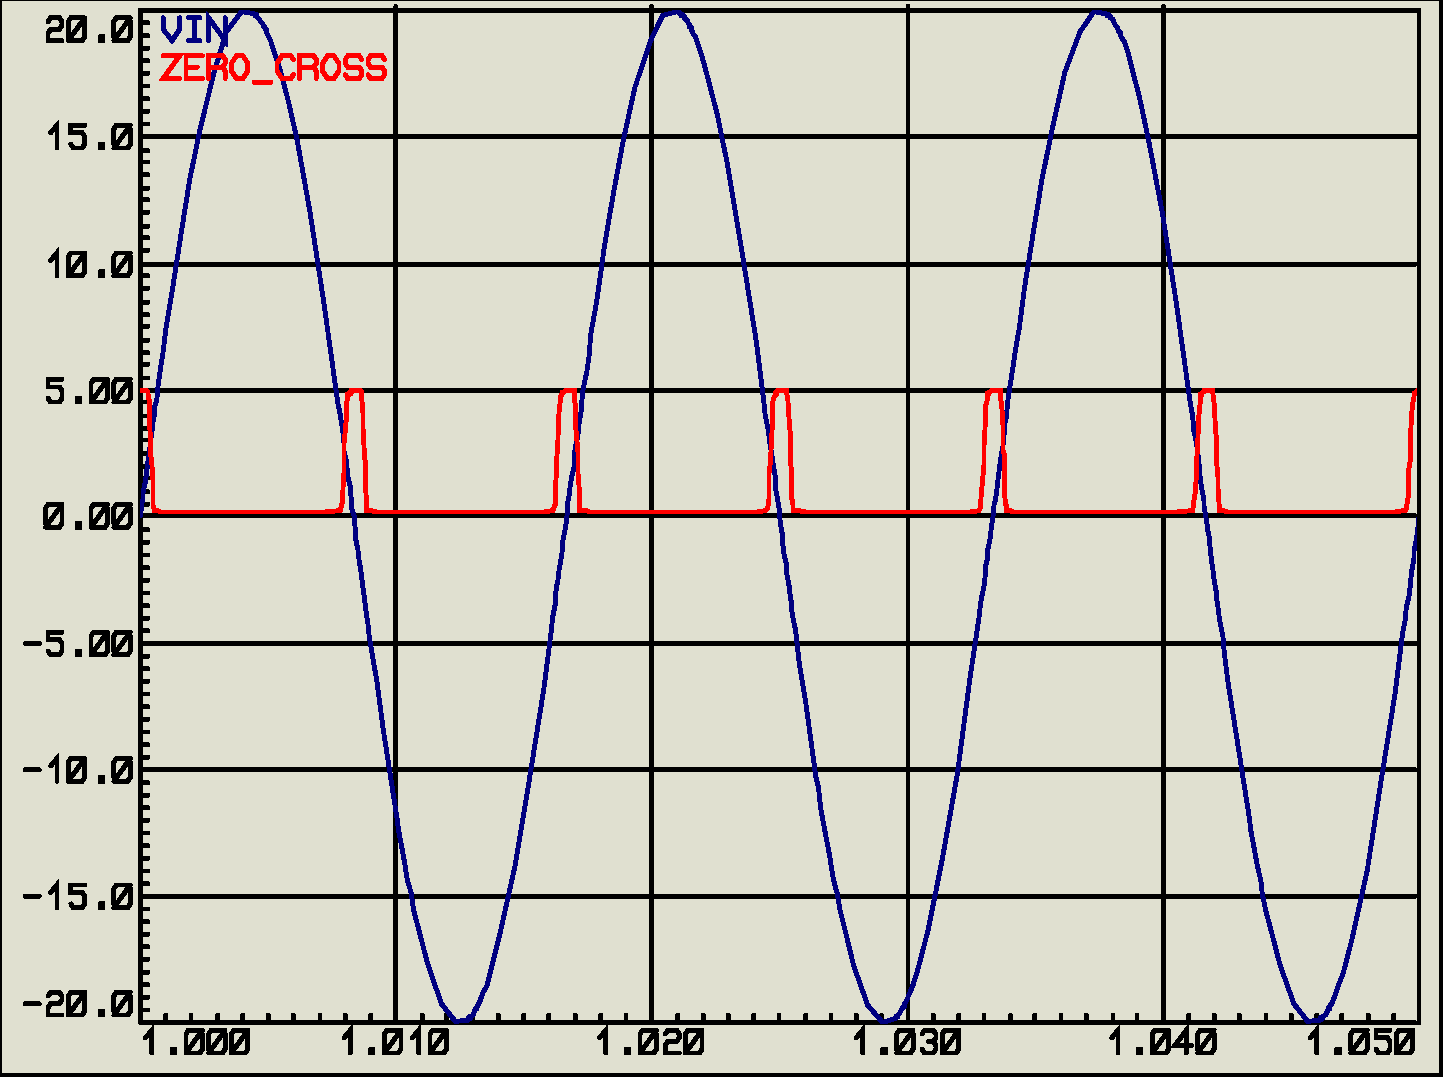
\includegraphics[width=\linewidth]{Figs/fig-008a.pdf}
\subcaption{Synchronization circuit output (in red) and power grid signal (in blue).}
\label{fig8a}
\end{minipage}
\hfill
\begin{minipage}[t]{0.47\textwidth}
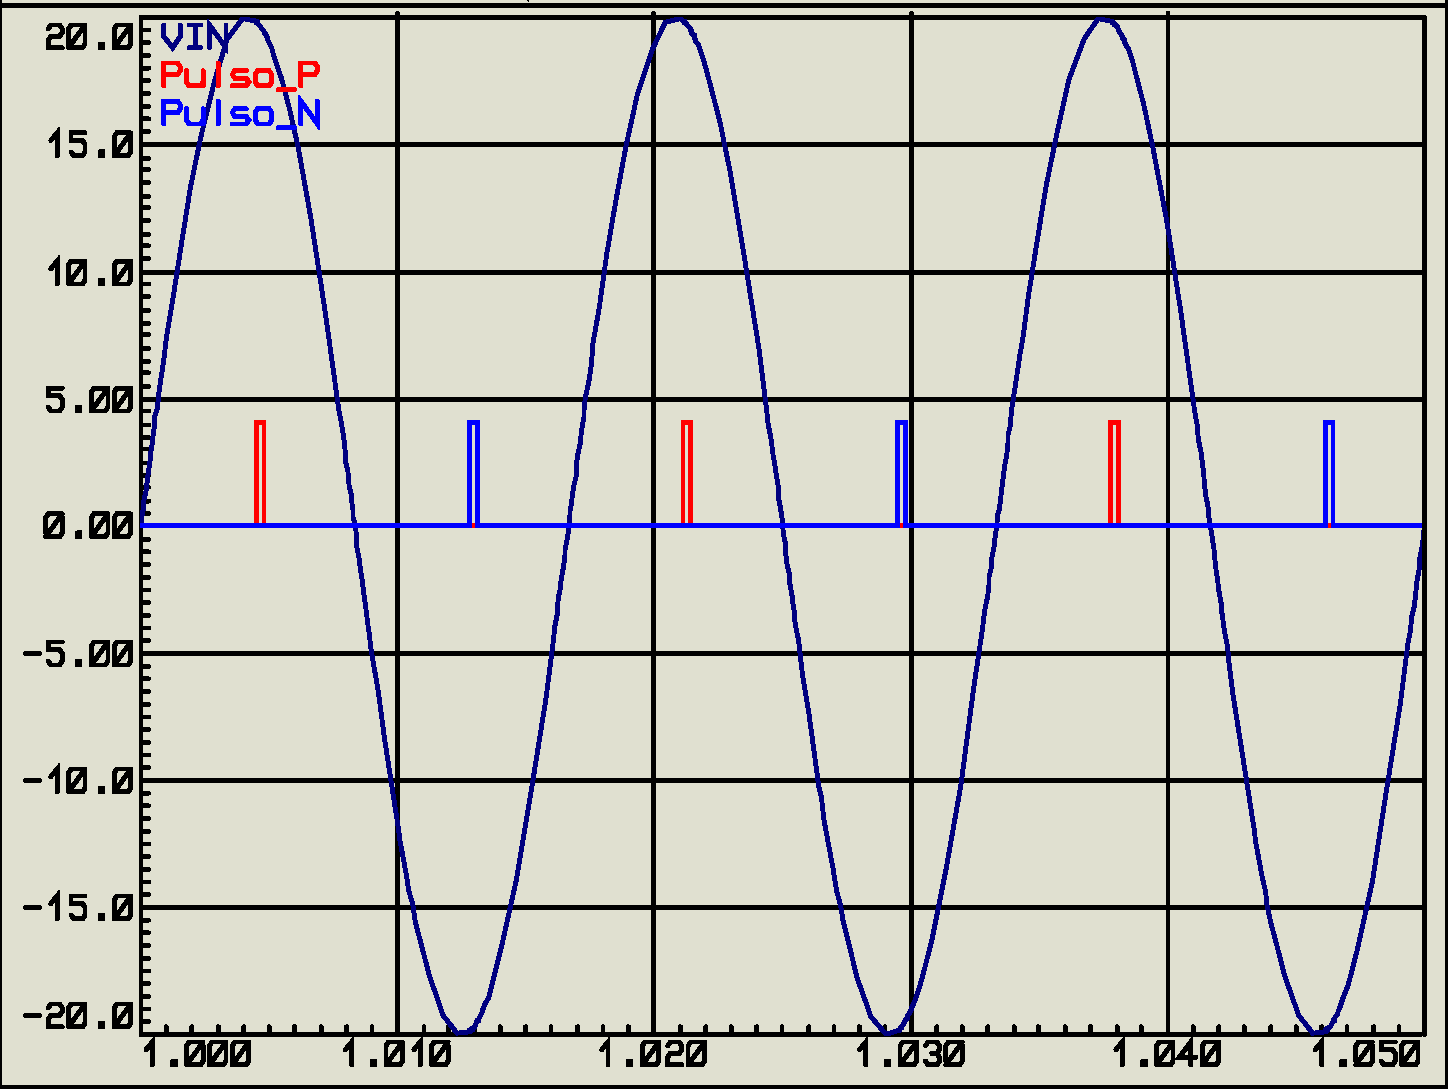
\includegraphics[width=\linewidth]{Figs/fig-008b.pdf}
\subcaption{Firing pulses generated by the microcontroller for the positive (in red) and negative half-cycle (in blue).}
\label{fig8b}
\end{minipage}
\vspace{0.5em} % Espaçamento vertical entre as linhas
% Segunda linha
\begin{minipage}[t]{0.47\textwidth}
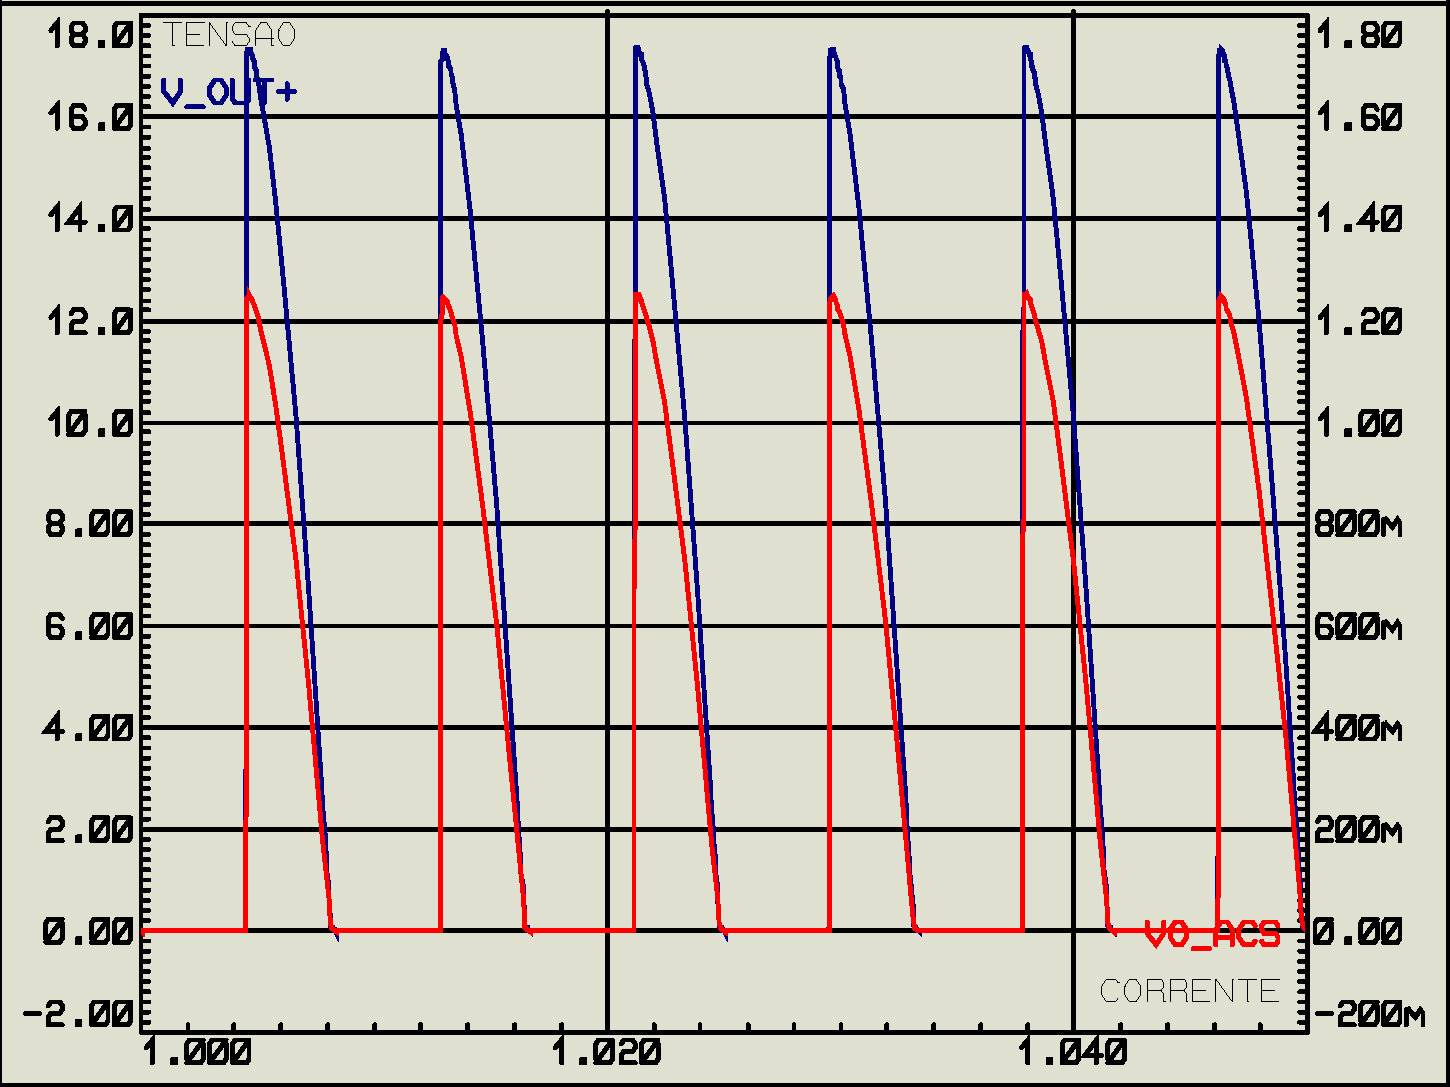
\includegraphics[width=\linewidth]{Figs/fig-008c.pdf}
\subcaption{Average current of $300$ mA (in red), firing angle of $90.72^{\circ}$.}
\label{fig8c}
\end{minipage}
\hfill
\begin{minipage}[t]{0.47\textwidth}
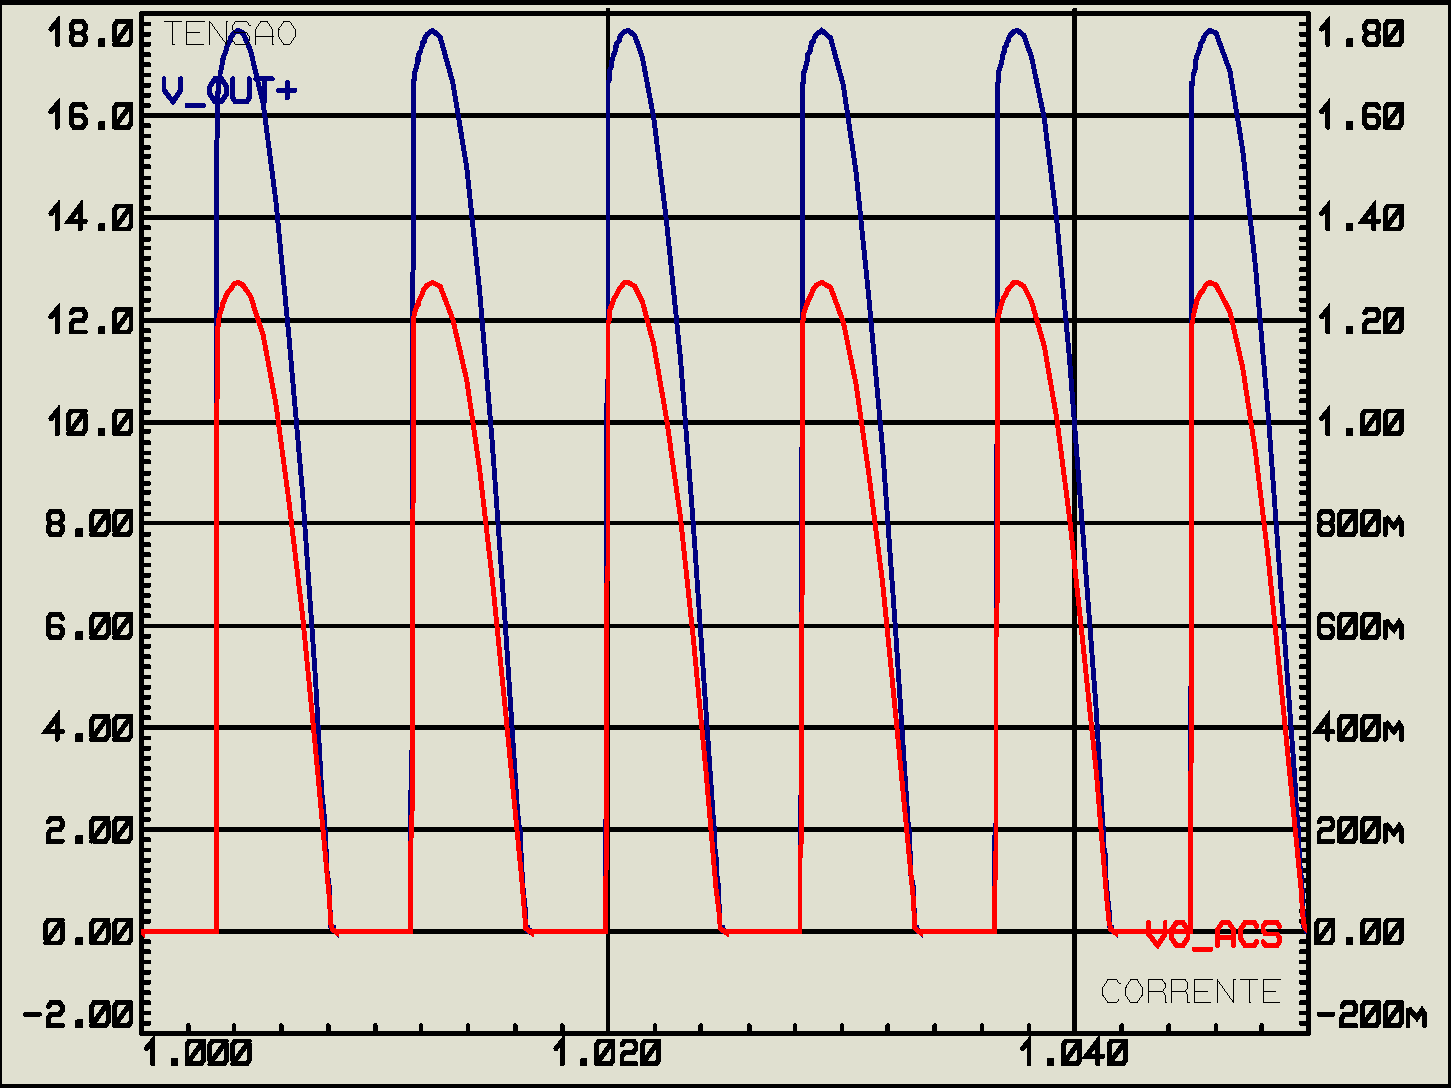
\includegraphics[width=\linewidth]{Figs/fig-008d.pdf}
\subcaption{Average current of $500$ mA (in red), firing angle of $43.2^{\circ}$.}
\label{fig8d}
\end{minipage}
\caption{Simulated results.}
\label{fig8}
\source{Own authorship.}
\end{figure}

\FloatBarrier
\subsubsection{Experimental results on the educational platform}
Figure \ref{fig9a} presents the experimental results from the synchronization and zero-crossing detection circuit, including the firing pulses generated by the microcontroller to trigger the thyristors. The voltage drop observed in Figure \ref{fig9b} results from the conduction threshold of the thyristors, which affects the input voltage of the educational platform. This behavior is expected due to the low operating voltage conditions—specifically, a peak voltage of 20V.

Figures \ref{fig9c} and \ref{fig9d} display the output voltage waveform across the load, along with the corresponding average output current values, measured using a multimeter. These results were obtained from the implementation of the closed-loop control algorithm.

\begin{figure}[t!]
\begin{minipage}[t]{0.48\textwidth}
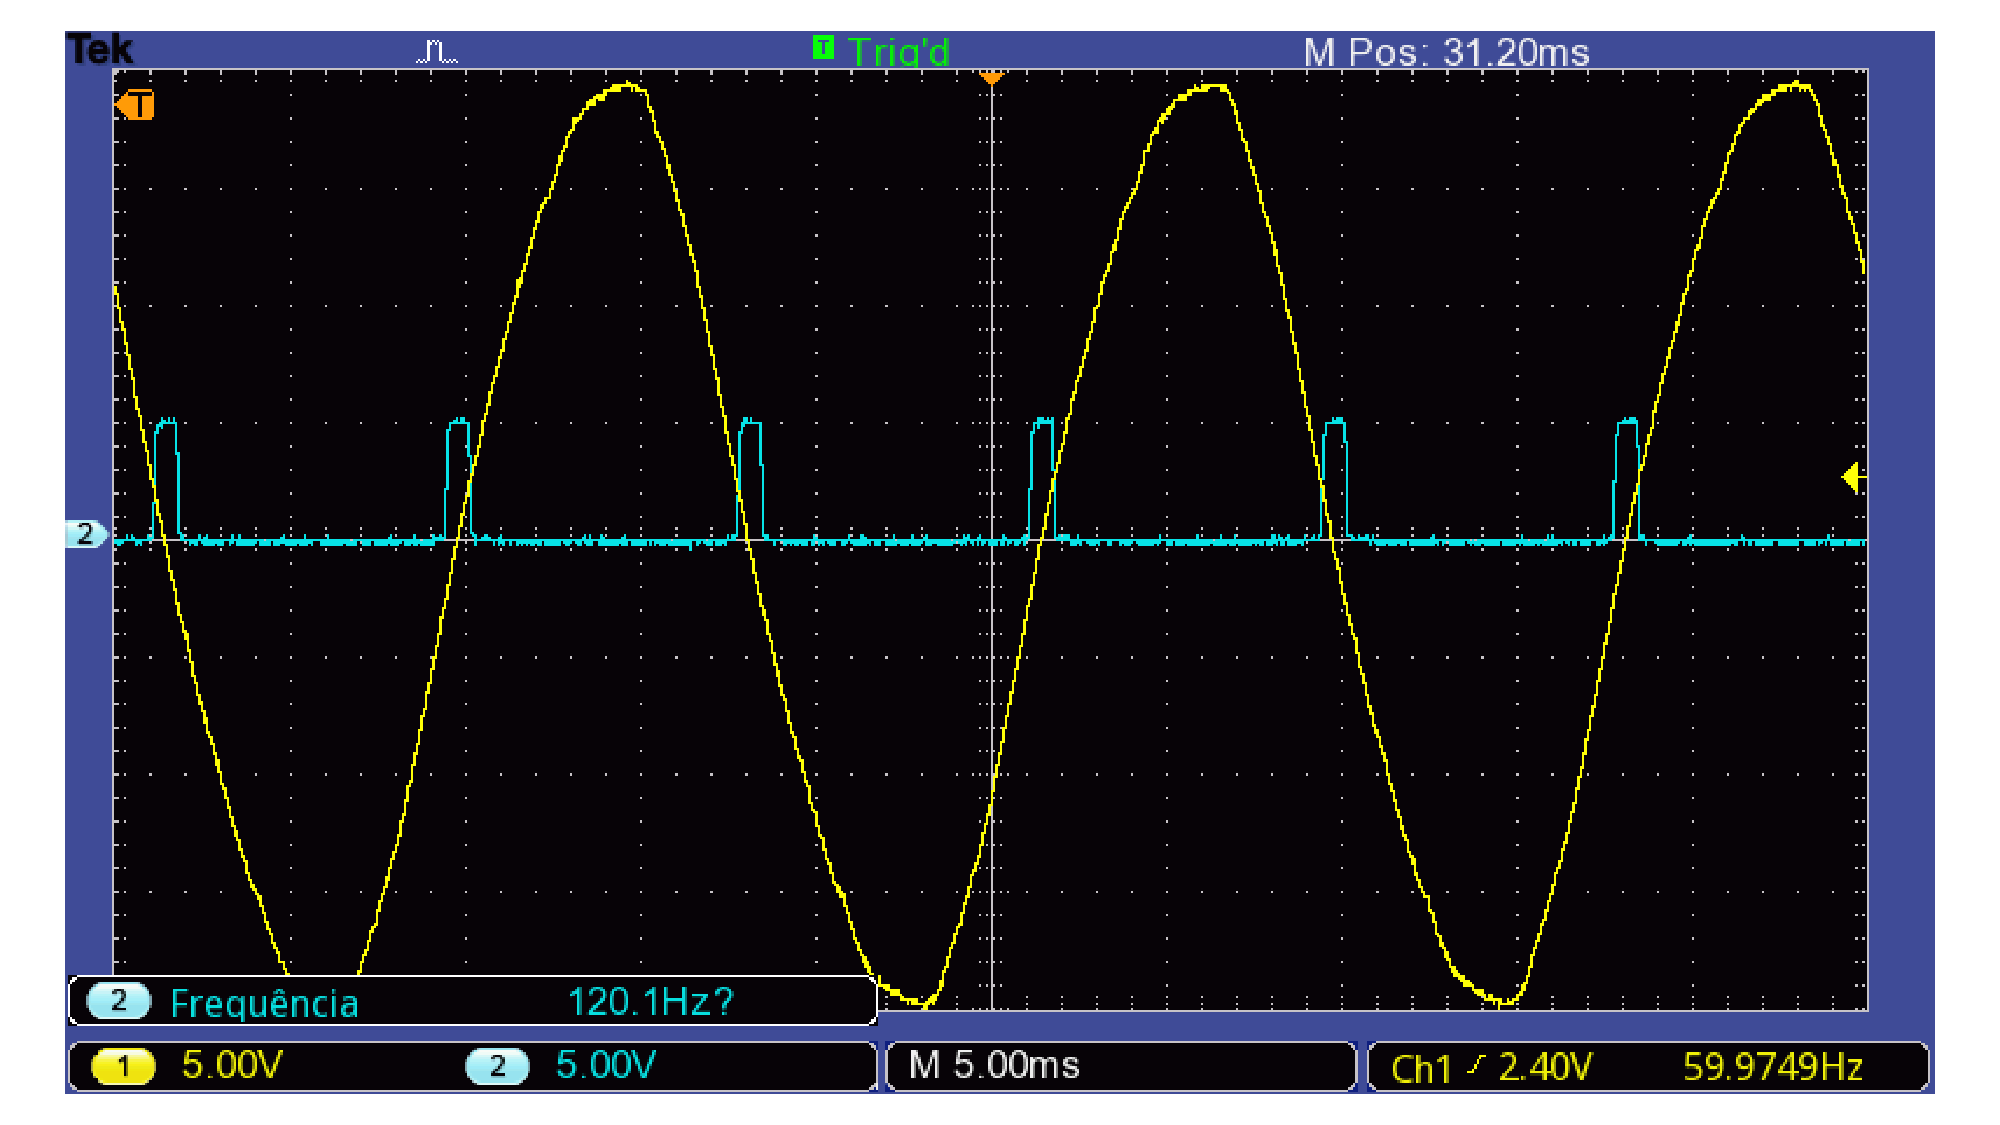
\includegraphics[width=\linewidth]{Figs/fig-009a.pdf}
\subcaption{Power grid signal (CH1 in yellow) and synchronization circuit output signal (CH2 in blue)}
\label{fig9a}
\end{minipage}
\hfill
\begin{minipage}[t]{0.48\textwidth}
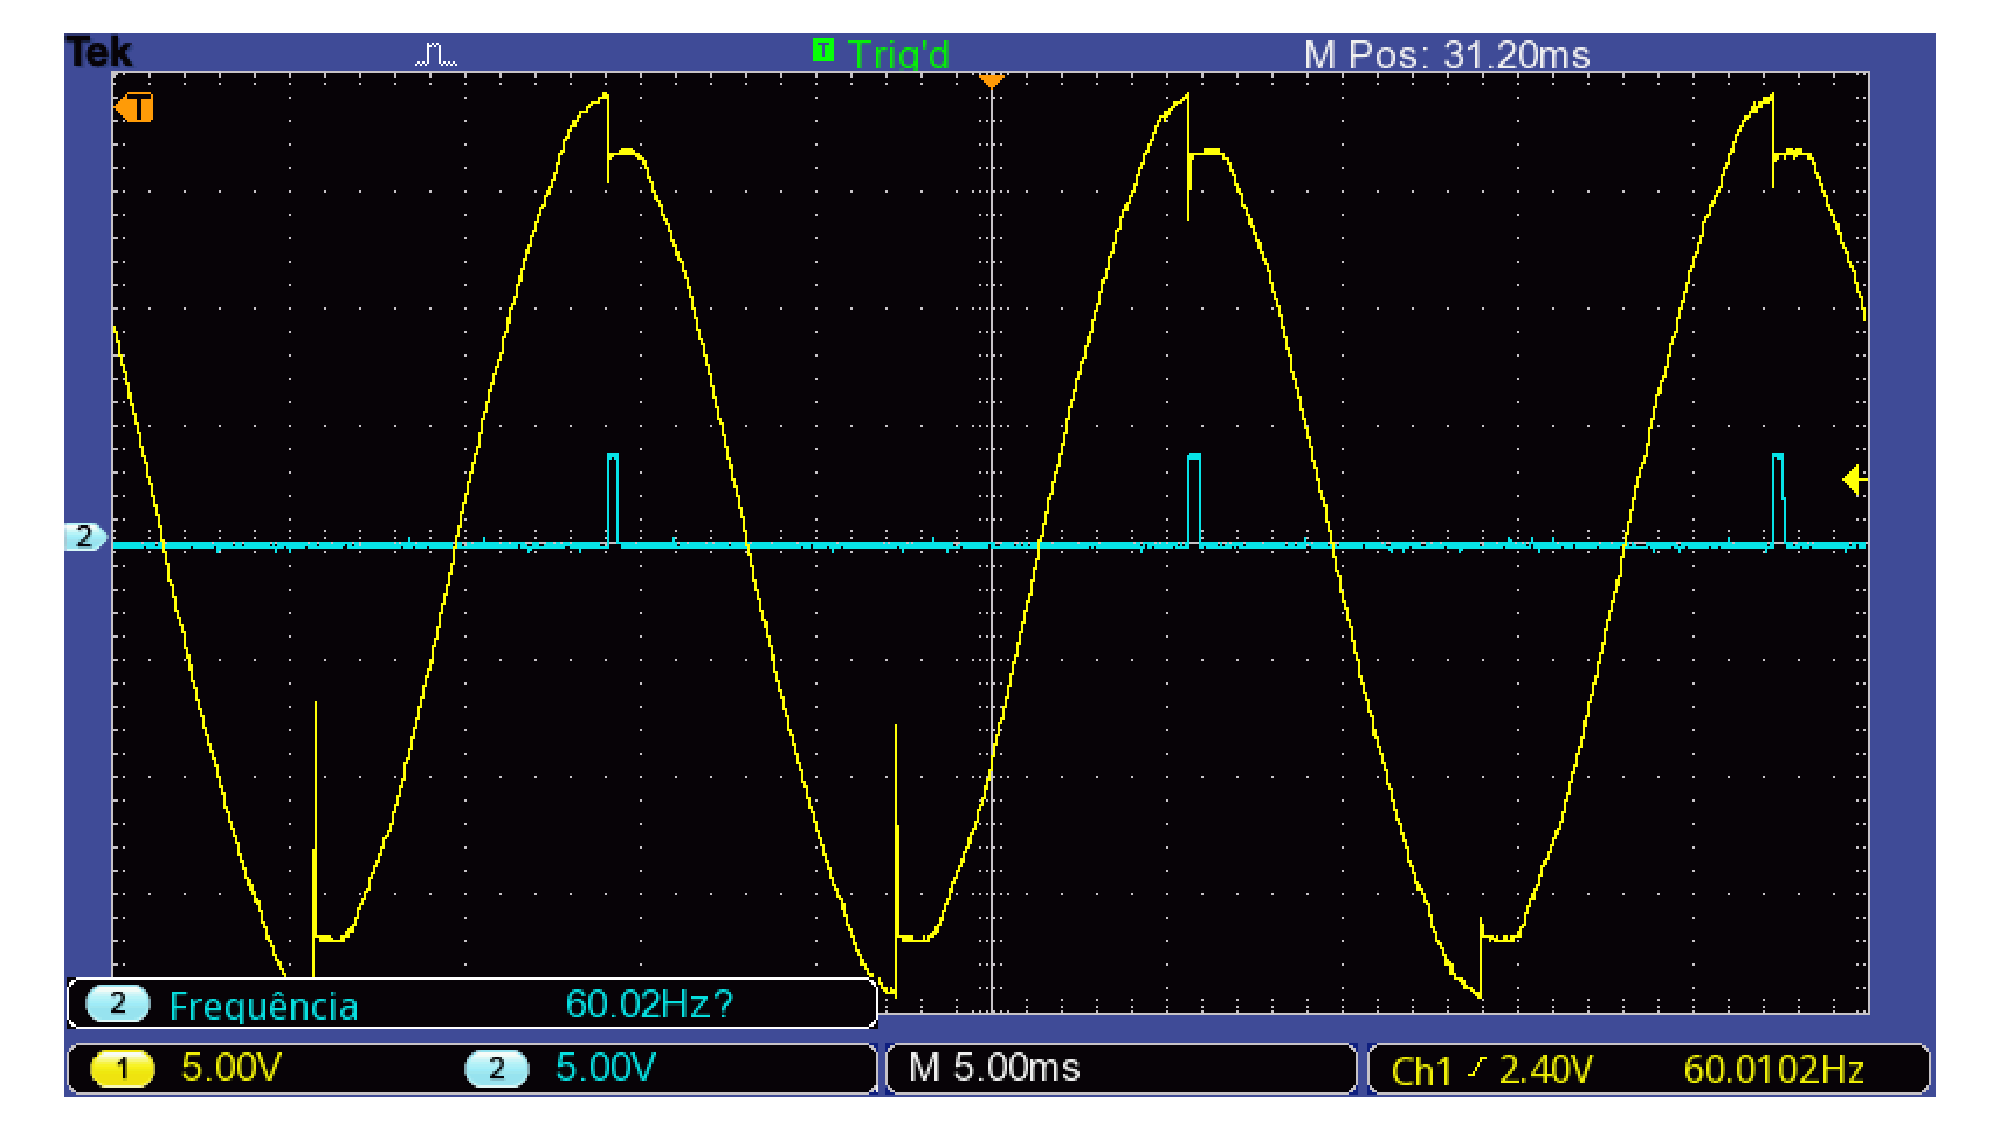
\includegraphics[width=\linewidth]{Figs/fig-009b.pdf}
\subcaption{Firing pulses generated by the microcontroller for the positive half-cycle (CH2 in blue).}
\label{fig9b}
\end{minipage}
\vspace{0.5em} % Espaçamento vertical entre as linhas
% Segunda linha
\begin{minipage}[t]{0.48\textwidth}
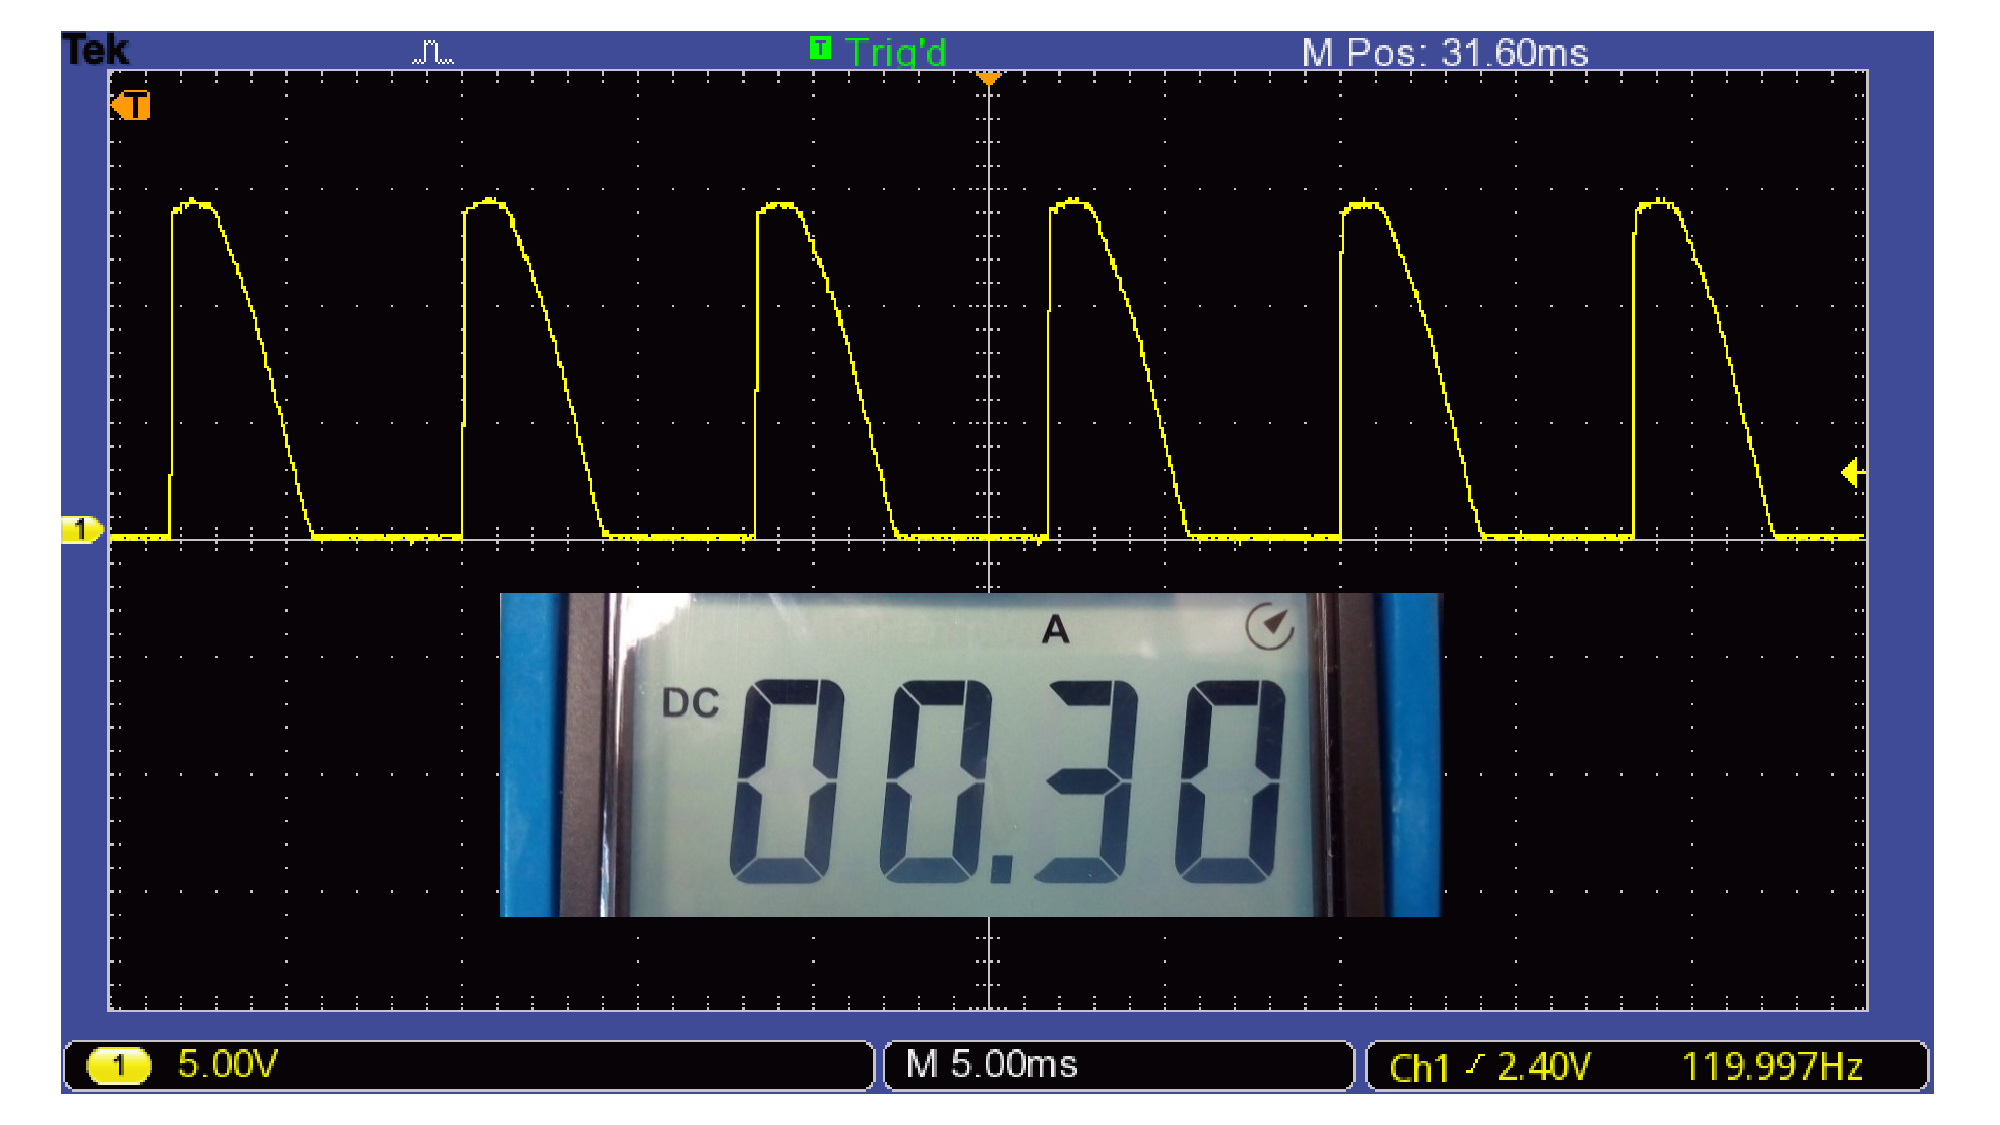
\includegraphics[width=\linewidth]{Figs/fig-009c.pdf}
\subcaption{Current waveform (CH1 in yellow) 
and indication of the value measured by a multimeter for a setpoint of $300$mA.}
\label{fig9c}
\end{minipage}
\hfill
\begin{minipage}[t]{0.48\textwidth}
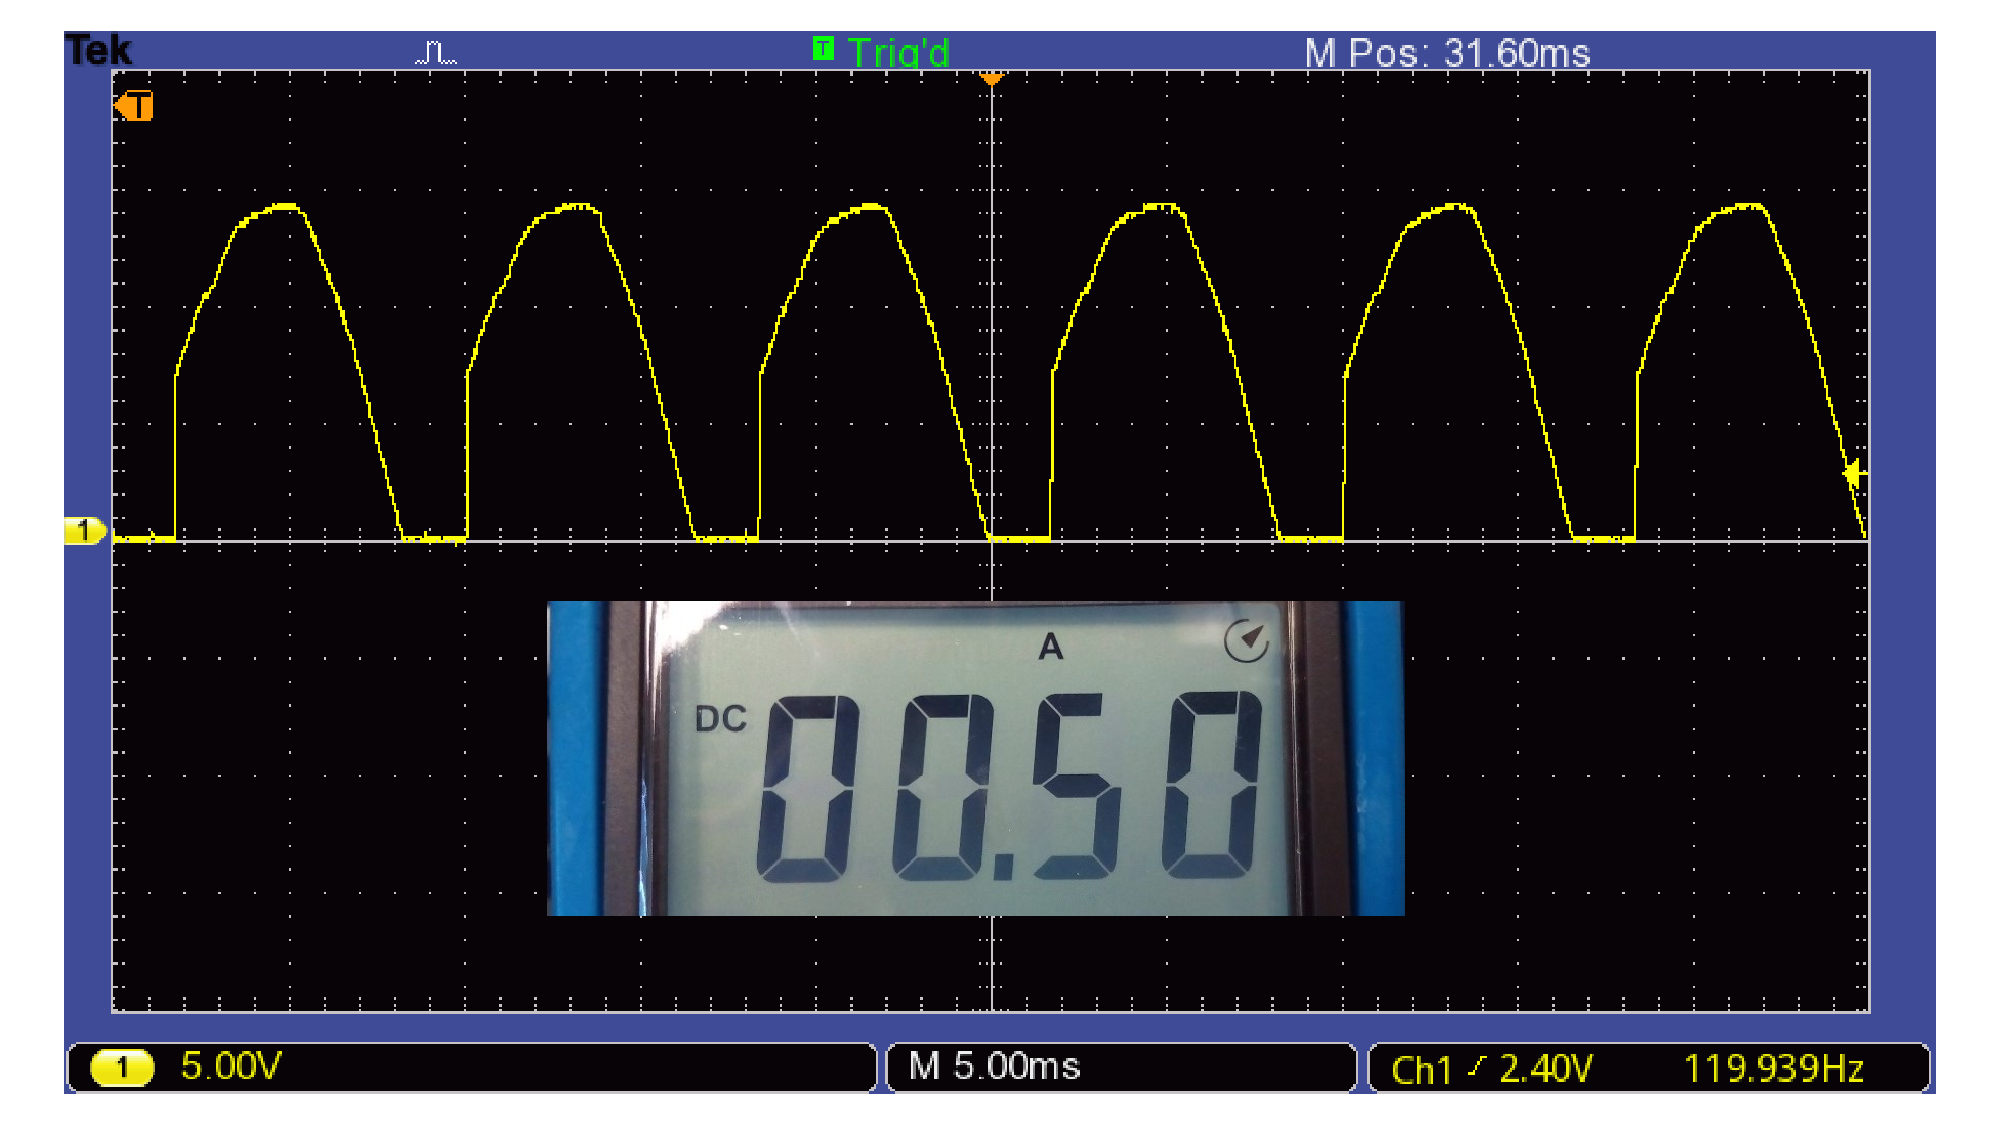
\includegraphics[width=\linewidth]{Figs/fig-009d.pdf}
\subcaption{Current waveform (CH1 in yellow) 
and indication of the value measured by a multimeter for a setpoint of $500$mA.}
\label{fig9d}
\end{minipage}
\caption{Experimental results.}
\label{fig9}
\source{Own authorship.}
\end{figure}


It is important to highlight that reference values of 300 mA and 500 mA were established for these tests. The measured output currents closely matched the desired values, thereby validating the effectiveness of the implemented closed-loop control strategy.

\subsection{Student feedback}
An analysis of student responses to questions Q1 through Q8 reveals a highly positive evaluation of the problem-based practical learning experience (Figure \ref{fig10}).     

\begin{figure}[h!]
\centering
\begin{minipage}{\textwidth}
 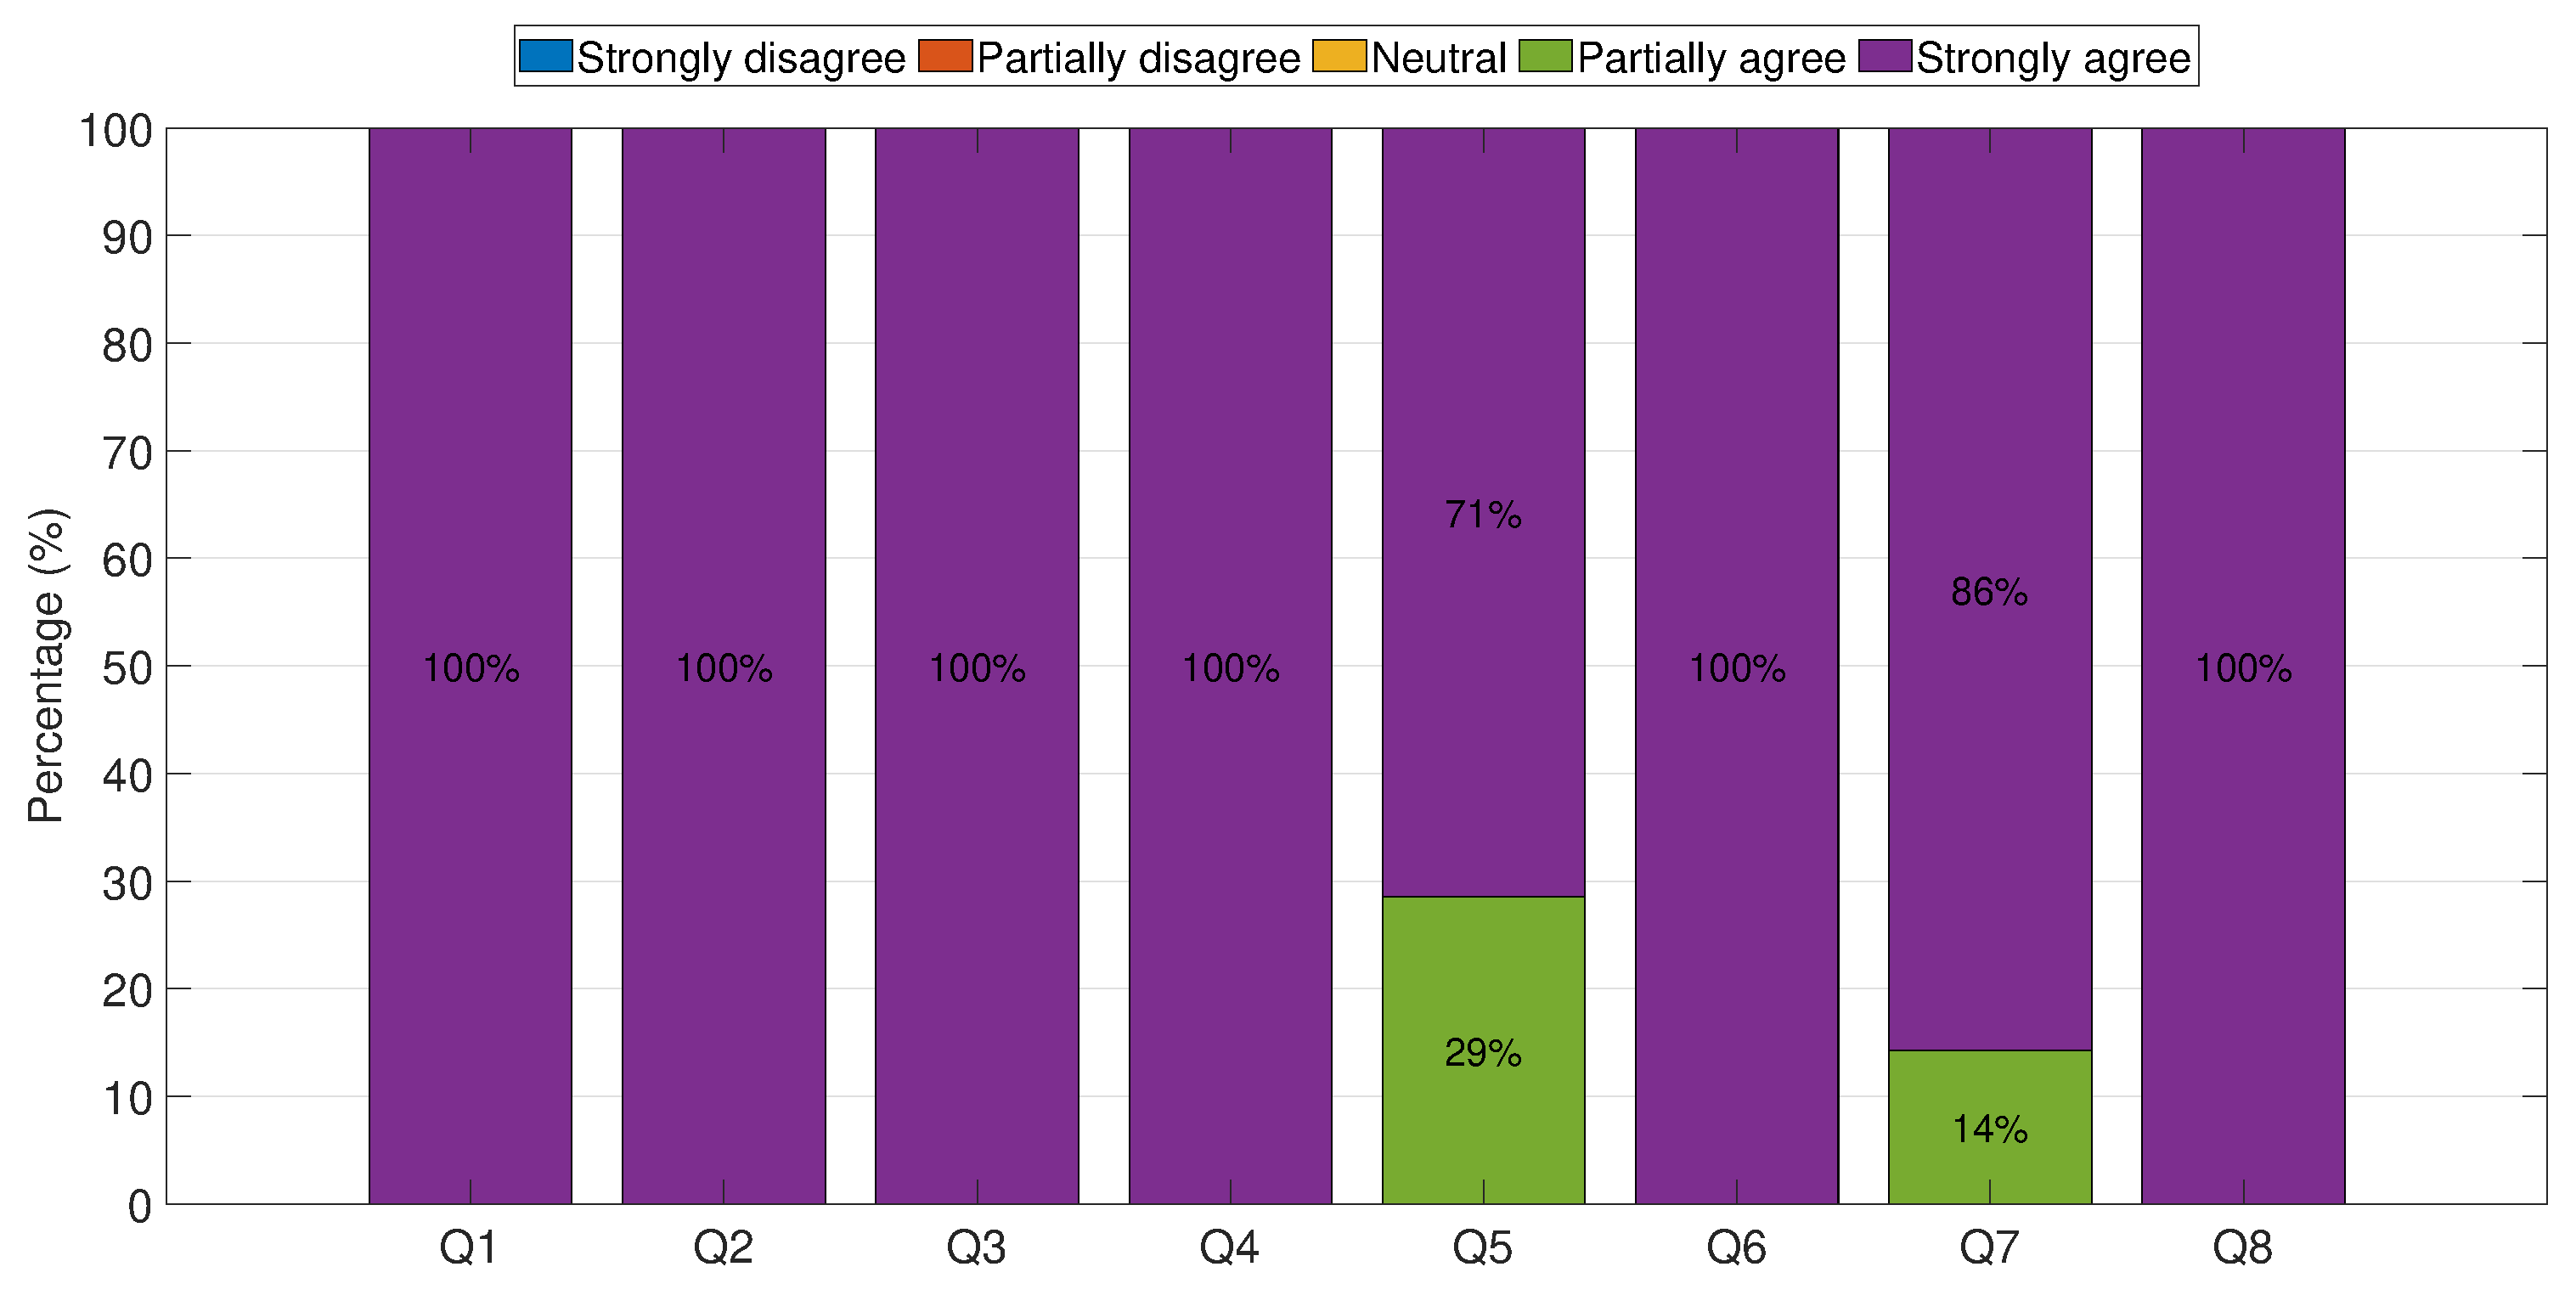
\includegraphics[width=\textwidth]{Figs/fig-010.eps}
 \caption{Distribution of student responses (in percentage) to questions Q1 to Q8 regarding the PBL methodology.}
 \label{fig10}
 \source{Own authorship.}
\end{minipage}
\end{figure}

Questions Q1 to Q4, which addressed engagement, satisfaction, and recommendation of the activity, received unanimous responses of ``strongly agree" (100\%), indicating a high level of motivation and approval of the pedagogical approach.

For questions Q5 to Q8, focused on the consolidation and application of theoretical knowledge, similarly high levels of agreement were observed. Questions Q6 and Q8 reached 100\% ``strongly agree", demonstrating the activity’s effectiveness in making abstract concepts more concrete and reinforcing understanding of digital control algorithm implementation.

Although slightly lower, the results for Q5 (71\% ``strongly agree", 29\% ``partially agree") and Q7 (86\% ``strongly agree", 14\% ``partially agree") still reflect a largely positive perception of the visualization and validation of theoretical concepts.

Overall, the findings confirm that the problem-based practical activity significantly contributed to student engagement and learning consolidation, with only minimal room for improvement in bridging theoretical knowledge with practical application.

\subsection{Cost-effective and scalable educational resource}

Given that many public institutions face financial constraints regarding investments in educational equipment, the platform proposed in this work presents a cost-effective alternative. Its accessibility lies in the low acquisition cost of the components required for assembly, as detailed in Table \ref{tbl-02}.

\begin{table}[htb]
\centering
\begin{threeparttable}
\caption{Estimated cost for acquiring the components of the educational platform.}
\label{tbl-02}
\begin{tabular}{p{5.3cm}cr}
\toprule 
Component    & Quantity [un]   & Cost (R\$)   \\ 
\midrule
Thyristor C106A & 4 & 12,60  \\ 
Diode 1N4007 & 8 & 0,96  \\ 
Integrated circuit MOC3021 & 4 & 10,04  \\ 
Optical coupler 4N25 & 1 &  1,71 \\ 
Resistor $120 \Omega$ & 8 & 0,72  \\ 
Resistor $470 \Omega$  & 3 & 0,27  \\
Resistor $10k \Omega$  & 1 &  0,09 \\ 
Resistor $15 \Omega$  & 1 & 0,09  \\ 
Potentiometer $10k \Omega$  & 1 & 2,20  \\ 
Current sensor ACS712-05B & 1 &  20,90 \\ 
Transformer $127V$/$12V$ & 1 & 28,00  \\ 
Phenolite board & 1 & 5,00  \\ 
\multicolumn{2}{l}{\textbf{Total}} & \textbf{82,58}  \\ 
\bottomrule
\end{tabular}
\source{Own authorship.}
\notes{Estimated cost in Brazilian national currency.}
\end{threeparttable}
\end{table}

The educational platform presented in this work enables the development of various competencies and skills essential for students in electrical, computer, electronic, control and automation, and mechatronics engineering programs. Ideally, the platform is intended for interdisciplinary use in practical laboratory sessions; however, it can also be used simultaneously across different courses to support the application of the concepts outlined in Figure \ref{fig11}.

\begin{figure}[h!]
\centering
\begin{minipage}{\textwidth}
 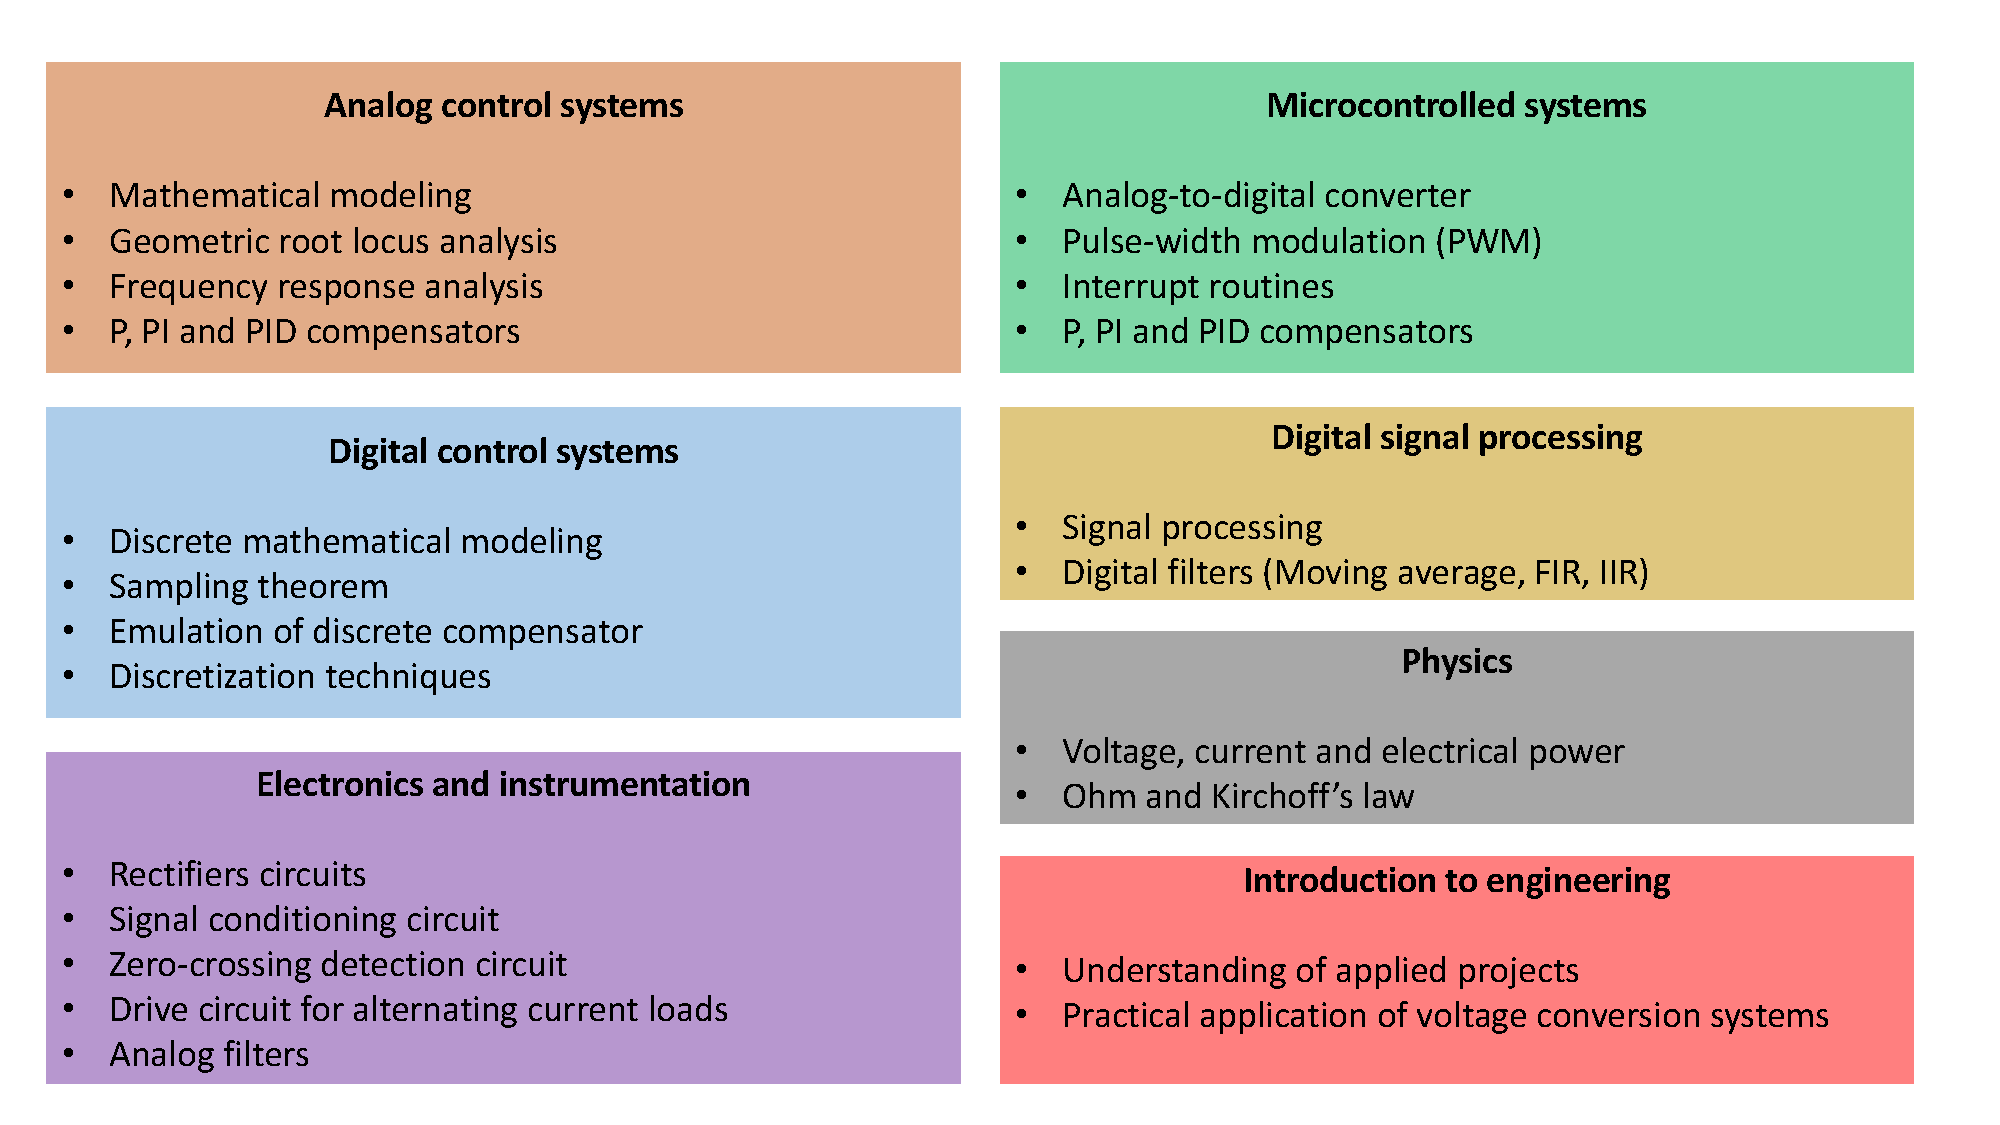
\includegraphics[width=\textwidth]{Figs/fig-011.pdf}
 \caption{Perspective of learning concepts that can be addressed in curricular units of engineering courses, aligned with the PBL methodology.}
 \label{fig11}
 \source{Own authorship.}
\end{minipage}
\end{figure}

In this study, a resistive load was employed, which is analogous to practical applications such as temperature control in an electric shower. However, the platform also allows for testing with other types of loads. For instance, a direct current (DC) motor could be used, where the thyristor firing angle is adjusted to maintain a constant rotational speed, even under varying load conditions on the shaft.

\FloatBarrier
\section{Conclusion}\label{sec-conclusao}

In this work, an open, low-cost educational platform for hands-on activities in power electronics, digital control, and embedded systems is presented and technically validated using a thyristor rectifier control application as a representative case study. The reported simulation and laboratory results are consistent with the expected theoretical behavior, supporting the feasibility and reliability of the proposed platform for implementing closed-loop control, acquiring relevant signals, and conducting repeatable experimental procedures under controlled conditions.

In addition to technical feasibility, the results suggest a positive educational contribution when the platform is deployed within a PBL activity. Student responses to the perception questionnaire indicate high levels of agreement regarding engagement, satisfaction, and willingness to recommend the activity, as well as perceived support for consolidating and applying theoretical concepts in digital control. While these findings are perception-based, they are consistent with the platform’s intended purpose of strengthening the theory–practice connection through an accessible and reproducible experimental environment.

To facilitate adoption and replication in engineering courses, a PBL workflow guideline is provided, including a suggested session plan and a concise rubric for grading technical artifacts. Together, these elements structure the iterative cycle of problem framing, modeling, implementation, and experimental validation, supporting consistent deployment across different course contexts.

Future work will expand the technical validation to additional application contexts and control strategies, as well as further enhance the platform in terms of modularity and instrumentation. Furthermore, the educational impact of implementing the platform in PBL activities can be investigated through studies involving a large number of students and utilizing objective learning measures.


\begin{english}
\printbibliography[title={References}]\label{sec-bib}
\end{english}
% if the text is not in Portuguese, it might be necessary to use the code below instead to print the correct ABNT abbreviations [s.n.], [s.l.]
%\begin{portuguese}
%\printbibliography[title={Bibliography}]
%\end{portuguese}


%full list: conceptualization,datacuration,formalanalysis,funding,investigation,methodology,projadm,resources,software,supervision,validation,visualization,writing,review

\begin{contributors}[sec-contributors]
\authorcontribution{Willian Ricardo Bispo Murbak Nunes}[conceptualization,datacuration,formalanalysis,funding,investigation,methodology,projadm,resources,software,supervision,validation,visualization,writing,review]
\authorcontribution{Rodrigo da Ponte Caun}[conceptualization,formalanalysis,methodology,validation,visualization,writing,review]
\authorcontribution{Winner Zavolski Queiroz}[datacuration,investigation,methodology,software,resources,validation,writing,review]
\end{contributors}

\begin{dataavailability}
\txtdataavailability{dataavailable} % options: dataavailable, dataonly, databody, datanotav, nodata
\end{dataavailability}

\end{document}

